\chapter{粲介子半轻单举衰变的数据处理与唯象学分析}
本章将系统性讨论D介子半轻单举衰变的唯象学分析。首先，对我国高能物理研究所的BESIII合作组和美国康奈尔大学的CLEO合作组测量$\mrm{D}$介子半轻单举衰变的实验现状进行介绍并讨论相关物理可观测量的抽取。其次，由于衰变宽度对重夸克质量高度敏感，本文将讨论三种不同的重夸克质量机制，分别是1S mass，$\overline{\mathrm{MS}}$ mass scheme和Pole mass scheme。对于唯象学分析，本文在三种质量方案下对非微扰参数进行了两种情形的全局拟合估计，分别是包含量纲三算符和五算符矩阵元贡献与包含量纲三算符，量纲五算符量纲六算符矩阵元贡献，并就非微扰参数的拟合估计结果进行讨论。最后定性讨论非微扰参数的拟合估计值对D介子寿命的影响。
\section{实验现状}
\subsection{D介子半轻单举衰变绝对分支比的实验测量}
CLEO合作组于2009年对三种$\mrm{D}$介子半轻衰变进行了测量\ct{CLEO:2009uah}。他们利用$e^{+}e^{-}$对撞，在质心能量$\mrm{E_{\mrm{cm}}}=3.774 \GeV$处积累了$818 \mathrm{pb}^{-1}$的$\mrm{D^{0}\overline{D^{0}}}$和$\mrm{D^{+} D^{-}}$事例，并测量了实验系下电子能谱$(\mrm{p_{e}>0.2\GeV})$和衰变分支比。此外，基于已知的遍举衰变数据对电子能谱$(\mrm{p_{e}>0.2\GeV})$进行红外端的外推，以测量$\mrm{D^{0}\to X e^{+}\nu}$和$\mrm{D^{+}\to X e^{+}\nu}$两个过程的电子能谱。对于$\mrm{D_s^+}$介子，他们在质心能量$\mrm{E_{\mrm{EM}}=4.170\GeV}$处积累了$602 \mrm{pb^{-1}}$的$\mrm{D_s^{*\pm}\mrm{D_s}^{\mp}}$事例，对$\mrm{D_s^{+}\to X e^{+}\nu}$的衰变分支比和电子能谱$(\mrm{p_{e}>0.2\GeV})$进行测量。并基于已知遍举衰变数据实现电子能谱的红外端外推，以获得该过程的电子能谱。CLEO合作组的测量结果为：

\begin{equation}
    \begin{aligned}
        \mathcal{B}\left(\mrm{D^0 \rightarrow X e^{+} \nu_e}\right)&=(6.46 \pm 0.09 \pm 0.11) \%,\\
        \mathcal{B}\left(\mrm{D^{+} \rightarrow X e^{+} \nu_e}\right)&=(16.13 \pm 0.10 \pm 0.29) \%,\\
        \mathcal{B}\left(\mrm{D_s^{+} \rightarrow X e^{+} \nu_e}\right)&=(6.52 \pm 0.39 \pm 0.15) \%,\\
    \end{aligned}
    \label{eq:CLEOBr}
\end{equation}
其中，两个误差分别是统计误差和系统误差。此外，他们讨论了D介子半轻单举过程$\mrm{SU(3)}$味道对称性的破坏，
$$
\begin{aligned}
    \Gamma\left(D^{+} \rightarrow X e^{+} \nu_e\right) / \Gamma\left(D^0 \rightarrow X e^{+} \nu_e\right)&=0.985 \pm 0.015 \pm 0.024,\\
    \Gamma\left(D_s^{+} \rightarrow X e^{+} \nu_e\right) / \Gamma\left(D^0 \rightarrow X e^{+} \nu_e\right)&=0.828 \pm 0.051 \pm 0.025,
\end{aligned}
$$
与理论预期基本相符。
\begin{figure}[htbp]
    \centering
    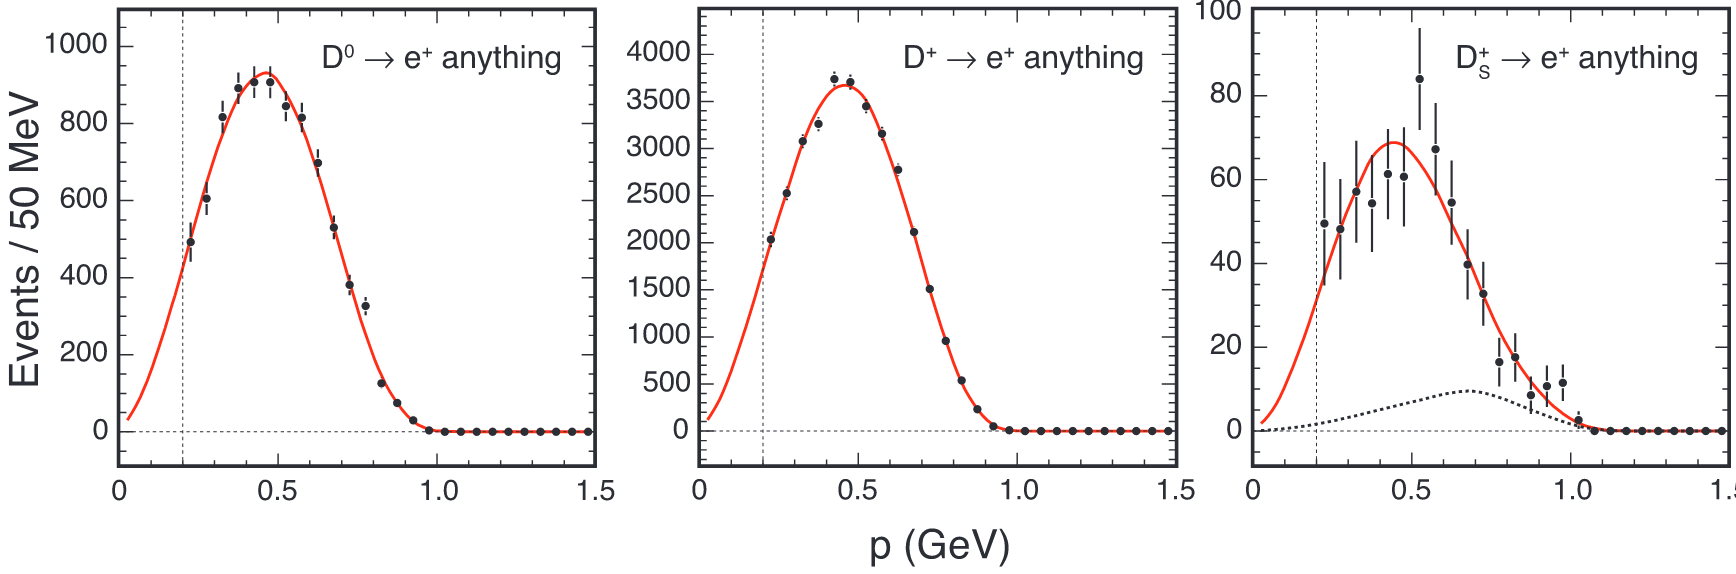
\includegraphics[width=1\textwidth]{figures/CLEOElectronsppart.png}
    \caption{实验室系下$\mrm{D}\to X e^+\nu$衰变过程的电子能谱\ct{CLEO:2009uah}}$\left(\mrm{p_{e}}> 0.2\GeV\right)$ % 添加图例
    \label{fig:cleo}  % 添加标签
\end{figure}
图\ref{fig:cleo}是CLEO合作组对$\mrm{D\to X e^+\nu}$过程电子能谱的测量结果,其中灰色垂直线表明电子的识别动量被截断于$0.2\GeV$处，误差棒仅包含统计误差。基于已知遍举衰变数据，红色实线是电子能谱的拟合结果。CLEO合作组提供了图\ref{fig:cleo}中对应每个bin的具体事例数和对应的统计误差，如表\ref{tab:cleo_electron_sp}所示，对于 $\mrm{D^{+}}$ 和 $\mrm{D_s^{+}}$，已经减除了来自轻子衰变 $\tau^{+} \nu_\tau$（ $\tau^{+} \rightarrow e^{+} \nu_e \bar{\nu}_\tau$）的贡献。结果表明 $\mrm{D^{0}}$与$\mrm{D^{+}}$介子的衰变电子能谱具有较高精度，但$\mrm{D_s^{+}}$介子的衰变电子能谱的精度较低。我国BESIII合作组于2021年重新抽取$\mrm{D_s^{+}}$介子的衰变电子能谱\ct{BESIII:2021duu}。
\begin{table}[h!]
    \centering
    \scriptsize  % 设置表格字体为小号
    \begin{tabular}{lrrr}
        \hline \hline
        $p(\mathrm{GeV})$ & $\Delta B\left(D^0 \rightarrow X e^{+} \nu_e\right)(\%)$ & $\Delta B\left(D^{+} \rightarrow X e^{+} \nu_e\right)(\%)$ & $\Delta B\left(D_s^{+} \rightarrow X e^{+} \nu_e\right)(\%)$ \\
        \hline 
        $0.200-0.250$ & $0.347 \pm 0.036$ & $0.912 \pm 0.040$ & $0.491 \pm 0.152$ \\
        $0.250-0.300$ & $0.426 \pm 0.030$ & $1.133 \pm 0.038$ & $0.470 \pm 0.124$ \\
        $0.300-0.350$ & $0.576 \pm 0.031$ & $1.379 \pm 0.041$ & $0.554 \pm 0.126$ \\
        $0.350-0.400$ & $0.629 \pm 0.030$ & $1.462 \pm 0.043$ & $0.515 \pm 0.120$ \\
        $0.400-0.450$ & $0.640 \pm 0.031$ & $1.675 \pm 0.047$ & $0.578 \pm 0.112$ \\
        $0.450-0.500$ & $0.640 \pm 0.031$ & $1.661 \pm 0.046$ & $0.562 \pm 0.123$ \\
        $0.500-0.550$ & $0.596 \pm 0.029$ & $1.546 \pm 0.044$ & $0.794 \pm 0.127$ \\
        $0.550-0.600$ & $0.575 \pm 0.029$ & $1.415 \pm 0.041$ & $0.611 \pm 0.115$ \\
        $0.600-0.650$ & $0.492 \pm 0.026$ & $1.243 \pm 0.038$ & $0.471 \pm 0.104$ \\
        $0.650-0.700$ & $0.374 \pm 0.023$ & $0.946 \pm 0.032$ & $0.314 \pm 0.087$ \\
        $0.700-0.750$ & $0.269 \pm 0.019$ & $0.674 \pm 0.026$ & $0.246 \pm 0.079$ \\
        $0.750-0.800$ & $0.230 \pm 0.017$ & $0.429 \pm 0.019$ & $0.089 \pm 0.060$ \\
        $0.800-0.850$ & $0.089 \pm 0.011$ & $0.240 \pm 0.014$ & $0.115 \pm 0.060$ \\
        $0.850-0.900$ & $0.053 \pm 0.008$ & $0.103 \pm 0.009$ & $0.037 \pm 0.046$ \\
        $0.900-0.950$ & $0.021 \pm 0.005$ & $0.022 \pm 0.004$ & $0.074 \pm 0.051$ \\
        $0.950-1.000$ & $0.002 \pm 0.002$ & $0.004 \pm 0.002$ & $0.096 \pm 0.045$ \\
        $1.000-1.050$ & $\cdots$ & $\cdots$ & $0.015 \pm 0.022$ \\
        \hline \hline
    \end{tabular}
    \caption{在实验室系下D介子半轻单举衰变过程每个bin的部分分支比\ct{CLEO:2009uah}}
    \label{tab:cleo_electron_sp}
\end{table}

%在我们接下来的唯象学分析中，对于$D_s^{+}$介子的衰变电子能谱，我们将使用BESIII合作组的测量结果，并在此基础上进行可观测量的抽取；对于$D^{0}$与$D^{+}$介子的衰变电子能谱，我们使用CLEO合作组的测量结果。

\subsection{$\mrm{D_s^+}$介子半轻单举衰变绝对分支比的实验测量}

BESIII合作组近期对$\mrm{D_s^{+}}$介子半轻单举衰变分支比进行测量\cite{BESIII:2021duu}。他们采用双标记技术在BEPCII对撞机上质心能量$\mrm{E_{\text{cm}} \in [4.178, 4.230] \ \mathrm{GeV}}$处产生的$\mrm{e^{+} e^{-}}$湮灭事例进行分析。主要包括：
\begin{itemize}
\item 2016年，在质心能量$\mrm{E_{\mathrm{cm}}}=4.178 \, \text{GeV}$处产生了$3.19 \, \mathrm{fb}^{-1}$的事例，$\mrm{e^{+} e^{-} \rightarrow D_s^{*+} D_s^{-}}$产生了大约$6.4 \times 10^6$个$\mrm{D_s^{+}}$介子，以及少量来自$\mrm{e^{+} e^{-} \rightarrow D_s^{+} D_s^{-}}$的贡献
\item 2017年，在质心能量$\mrm{E_{\mathrm{cm}}}\in [4.189, 4.219]\GeV$处产生了$2.08 \, \mathrm{fb}^{-1}$的事例
\item 2013年，在质心能量$\mrm{E_{\mathrm{cm}}}\in [4.225, 4.230 ]\GeV$内收集的$1.05 \, \mathrm{fb}^{-1}$的事例
\end{itemize}

有关$\mrm{D_s^+}$半轻单举衰变绝对分支比和该过程$\mrm{SU(3)}$对称性破坏的测量结果为：
\begin{equation}
    \begin{aligned}
     \mathcal{B}\left(\mrm{D_s^{+} \rightarrow X e^{+} \nu_e}\right) 
    &=(6.30 \pm 0.13(\text { stat. }) \pm 0.09(\text { syst. }) \pm 0.04(\text { ext. })) \%,\\
         \frac{\Gamma\left(\mrm{D_s^{+} \rightarrow X e^{+} \nu_e}\right)}{\mrm{\Gamma\left(D^0 \rightarrow X e^{+} \nu_e\right)}} 
         &=0.790 \pm 0.016 \text { (stat.) } \pm 0.011 \text { (syst.) } \pm 0.016 \text { (ext.). }\\
    \end{aligned}
         \label{eq:BESIIIGamma__Br_Ds}  
        \end{equation}
式\eqref{eq:BESIIIGamma__Br_Ds}中的误差分别是统计误差，系统误差以及电子动量$\mrm{p_e<0.2\GeV}$区域的外推误差。该结果与CLEO合作组的测量结果基本一致，但BESIII合作组的测量精度更高。$\mrm{D_s}$介子半轻单举衰变宽度与$\mrm{D^0}$介子半轻单举衰变宽度的比值偏离1反映了$\mrm{SU(3)}$味道对称性的破坏。

此外，BESIII合作组基于已知遍举衰变数据对测量得到部分电子能谱进行红外端($\mrm{p}_{e}<0.2\GeV$的区域)外推，如图\ref{fig:BESIIIElectrons}所示，其中黑色带误差棒的点表示每个bin内的事例数，蓝色曲线表示拟合结果。结果表明，BESIII合作组的测量结果与CLEO合作组的测量结果基本一致。
\begin{figure}[htbp]
    \centering
    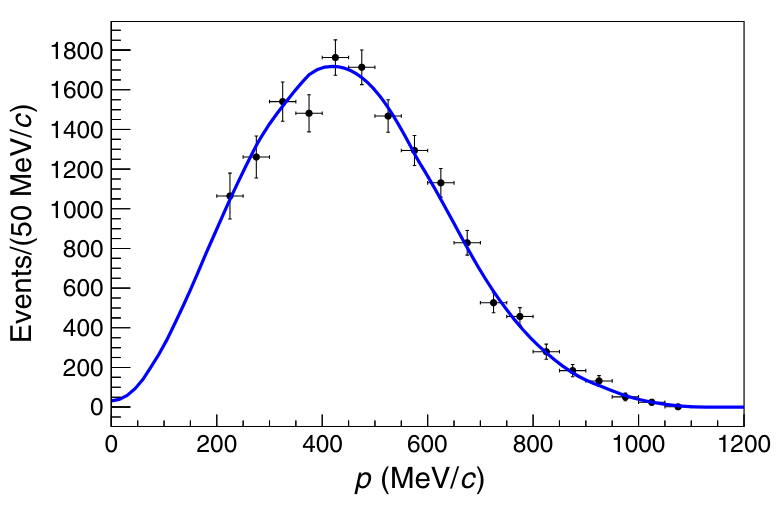
\includegraphics[width=0.6\textwidth]{figures/BESIIIElectrons.png}
    \caption{实验室系下$\mrm{D_s^+\to X e^+\nu}$衰变过程的电子能谱\ct{BESIII:2021duu}}$\left(\mrm{p_{e}}> 0.2\GeV\right)$ % 添加图例
    \label{fig:BESIIIElectrons}  % 添加标签
\end{figure}
此外，BESIII合作组也提供了$\mrm{D_s^+}\to X e^+\nu$过程（图\ref{fig:BESIIIElectrons}）对应每个bin的具体事例数与相应的统计误差（表\ref{tab:BESIII_Ds_electron_sp}），其中双标记侧产额已经经过效率修正和背景减除。

    \begin{table}[htbp]
        \centering  % 确保表格居中
        \scriptsize  % 表格文字变小
        \begin{tabular}{cccccccc}
            \hline
            \hline
            $\mrm{p_e}(\mathrm{MeV} / c)$ & $N_{DT, X e^{+}\nu}$ &$\mrm{p_e}(\mathrm{MeV} / c)$ & $N_{DT, X e^{+}\nu}$ & $\mrm{p_e}(\mathrm{MeV} / c)$ & $N_{DT, X e^{+}\nu}$ & $\mrm{p_e}(\mathrm{MeV} / c)$ & $N_{DT, X e^{+}\nu}$ \\
            \hline
            $200-250$ & $1064 \pm 115$ & $450-500$ & $1713 \pm 88$ & $700-750$ & $526 \pm 51$ & $950-1000$ & $52 \pm 19$ \\
            $250-300$ & $1261 \pm 106$ & $500-550$ & $1468 \pm 82$ & $750-800$ & $457 \pm 44$ & $1000-1050$ & $24 \pm 14$ \\
            $300-350$ & $1540 \pm 99$ & $550-600$ & $1294 \pm 76$ & $800-850$ & $280 \pm 38$ & $1050-1100$ & $2 \pm 6$ \\
            $350-400$ & $1482 \pm 93$ & $600-650$ & $1130 \pm 72$ & $850-900$ & $184 \pm 31$ & -&- \\
            $400-450$ & $1762 \pm 90$ & $650-700$ & $829 \pm 62$ & $900-950$ & $132 \pm 27$ & -&- \\
            \hline
            \hline
        \end{tabular}
        \caption{实验室系下$\mrm{D_s^+}$介子半轻单举衰变过程双标记侧每个bin的产额\ct{BESIII:2021duu}}
        \label{tab:BESIII_Ds_electron_sp}
    \end{table}
\section{唯象学分析}
本节利用表\ref{tab:cleo_electron_sp}和表\ref{tab:BESIII_Ds_electron_sp}的数据，基于重夸克有效理论，对电子能谱的红外区域进行拟合外推并重新抽取其衰变宽度和分支比。此外，本节利用蒙特卡洛方法(Monte Carlo, MC)抽取$\mrm{D\to X e^+ \nu}$过程的电子能量原点矩。 通过洛伦兹变换将其变换至D介子质心系并讨论其关联效应。
\subsection{电子能谱红外区域的理论外推}
CLEO合作组于2009年给出实验室系下$\mrm{D\to X e^+ \nu_e}$的电子能谱($\mrm{p_{e}>0.2\GeV}$)，在$p_{e}<0.2\GeV$区域，由于重夸克有效理论的算符乘积展开不存在奇异行为，因此本文用谱的理论形式拟合前四个bin的数据，并将其外推至$\mrm{p_{e}<0.2}\GeV$区域。
\begin{equation}
    \frac{\mrm{d} \Gamma}{  \mrm{d} E_{e}}=\Gamma_{0} a (\frac{2}{m_{c}})^3 E_{e}^{2}(1+ b\frac{2E_{e}}{m_{c}})(1-\frac{2E_{e}}{m_{c}}),
    \label{func:fitting function}
    \end{equation}
其中$m_{\mrm{c}}$是粲夸克质量，$a,b$是拟合参数,$\Gamma_{0}=\frac{G_{F}^2 m_{c}^5(V_{cd}^2+V_{cs}^2)}{192\pi^3}$。本文以$\mrm{D^{0}}$介子为例讨论红外区域的拟合外推。

为实现更优的拟合效果，并使之与表\ref{tab:cleo_electron_sp}中前四个bin的数据保持一致，需要在理论模型中引入一个标度因子，该因子包括$\mrm{D^{0}}$介子寿命以及相应的量纲转换因子g。
\begin{equation}
    \Delta Br_{i}= \frac{\Delta \Gamma_{i}}{\Gamma}=\frac{1}{\Gamma} \frac{\mrm{d}\Gamma}{\mrm{d}x}dx==\frac{1}{\Gamma} \frac{\mrm{d}\Gamma}{\mrm{d}x}\Delta x_{i}=g\tau_{\mrm{D^{0}}}\frac{\mrm{d}\Gamma}{\mrm{d}x}\Delta x_{i}, 
\end{equation}
其中，指标$i$是每个bin的编号，$m_{\mrm{c}}\Delta x_{i}/2$是电子能量的bin宽度。$\tau_{\mrm{D^{0}}}$是$\mrm{D^{0}}$介子寿命，为$410.3\pm1.5 10^{-15}s$;粲夸克质量采取$\overline{\mrm{MS}}$质量方案，$m_{c}=\overline{\mrm{m}}_{c}(1.27\GeV)=1.27\GeV$，$\mrm{V_{cs}}=0.975,\mrm{V_{cd}}=0.221$。

定义$\chi^{2}$函数如下
\begin{equation}
    \chi^{2}=\sum_{i=1}^{4}(\frac{\Delta Br_{i,\text{theory}}-\Delta Br_{i,\text{exp}}}{\Delta Br_{i,\sigma}})^2,
\end{equation}
其中$\Delta Br_{i,\sigma}$是每个bin分支比的标准误差，$\Delta Br_{i,\text{theory}}$是每个bin的理论预言值，$\Delta Br_{i,\text{exp}}$是每个bin的实验观测中心值。
拟合结果表明：$\chi^{2}_{min}=1.2618, a\to \hat{a}=0.49, b\to \hat{b}=0.40$.
表\ref{tab:cleo_electron_sp}前四个bin数据的误差最终体现于拟合参数$\hat{a},\hat{b}$的拟合估计误差。
\begin{equation}
    \left(\boldsymbol{V}^{-1}(\hat{\boldsymbol{\theta}})\right)_{i j}=\left[\frac{1}{2} \frac{\partial^2 \chi^2}{\partial \theta_i \partial \theta_j}\right]_{\boldsymbol{\theta}=\hat{\boldsymbol{\theta}}} \quad i, j=1,2, \cdots, k .
    \label{eq:cov_CLEO_D0_exp}
    \end{equation}
式\eqref{eq:cov_CLEO_D0_exp}中, $\mrm{V}$是拟合模型里参数的协方差矩阵，$\theta$是理论模型中的参数，$\hat{\theta}$是理论模型中的参数的拟合估计值。 对拟合参数的协方差矩阵进行平方根运算，此时矩阵的对角元是拟合参数的标准误差。拟合结果表明：

$$\chi^{2}_{min}=0.6,\quad a\to \hat{a}=0.49(12),\quad b\to \hat{b}=0.40(57).$$

考虑到拟合曲线在每个bin内的非线性行为，基于式\eqref{func:fitting function}对表\ref{tab:cleo_electron_sp}中前四个bin的数据在积分意义上进行标度转换，以将其映射至$\mrm{p_{e}<0.2\GeV}$,

\begin{equation}
    \Delta \text{Br}[i] = \frac{\int_{0.05 i}^{0.05(i+1)} g \tau_{D^{0}} \frac{\mathrm{d} \Gamma}{ \mathrm{d} E_{\mathrm{e}}} \, \mathrm{d} E_{\mathrm{e}}}{\int_{0.2}^{0.4} g \tau_{D^{0}} \frac{\mathrm{d} \Gamma}{ \mathrm{d} E_{\mathrm{e}}} \, \mathrm{d} E_{\mathrm{e}}}, \quad i = 1, 2, 3, 4.
    \label{eq:scaled}
\end{equation}
电子能量位于0到$0.2\GeV$区域的数据如表\ref{tab:cleo_electron_sp_fit}所示，
\begin{table}[htbp]
    \centering
\begin{tabular}{llll}
    \hline\hline
    $E_{e}/\GeV$& $\Delta B\left(D^0 \rightarrow X e^{+} \nu_e\right)(\%)$&$E_{e}/\GeV$& $\Delta B\left(D^0 \rightarrow X e^{+} \nu_e\right)(\%)$\\
    \hline
    0-0.05 & $0.0072 \pm 0.0015$ & 0.1-0.15 & $0.122 \pm 0.016$ \\
    0.05-0.1 & $0.048 \pm 0.008$ & 0.15-0.2 & $0.222 \pm 0.021$\\
    \hline\hline
\end{tabular}
\caption{$\mrm{D^{0}}$介子半轻单举衰变电子能谱红外区域外推结果}
\label{tab:cleo_electron_sp_fit}
\end{table}

    CLEO合作组在衰变分支比的水平上给出了相应统计误差和系统误差，即
    \begin{equation}
    \mathcal{B}\left(\mrm{D^0 \rightarrow X e^{+} \nu_e}\right)=(6.46 \pm 0.09 \pm 0.11) \%,
    \end{equation}
   出于保守考虑, 本文假设每个bin的系统误差与中心值的比值相同，即各个bin之间的系统误差完全相关。由于CLEO合作组并未提供各个bin的具体系统误差，本文采用一种简化方法，将衰变分支比中系统误差与中心值的比值延拓至电子能量bin的水平。即每个bin的系统误差与中心值比值被假设为一个固定值且与衰变分支比中该比值保持一致。

   具体地，基于蒙特卡洛技术以0为中心值、0.11/6.46作为标准误差生成一组衰变分支比水平上系统误差与中心值的比值，这组比值有200000个点。假设每个bin的分支比服从正态分布，以每个bin的右端点作为中心值,系统误差作为标准误差生成一个$20\times 200000$数据集。每个bin的每格数据点与其系统误差带来的扰动相加和，可得$\mrm{D^{0}}$介子半轻单举衰变电子能谱的数据集。该数据集的每个电子能量bin包含200000个服从正态服从的数据点，且该正态分布的标准误差同时包含系统误差和统计误差。
\begin{figure}[htbp]
    \centering
    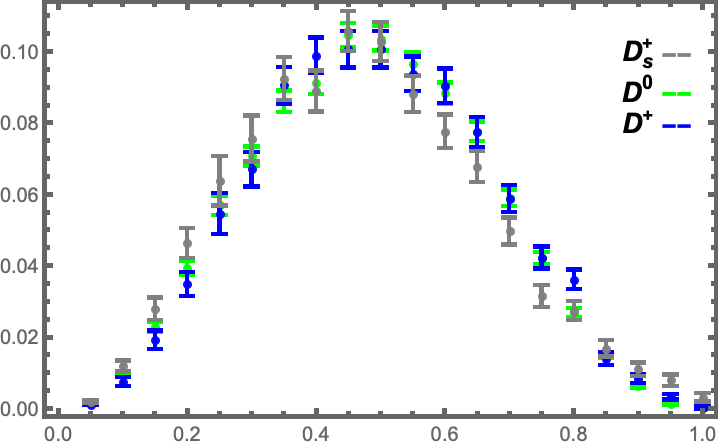
\includegraphics[width=0.8\textwidth]{figures/Dspectrum.png}
    \caption{实验室系下$\mrm{D}\to X e^+\nu_e$衰变过程归一化的电子能谱} % 添加图例
    \label{fig:cleo_D_sp}  % 添加标签
\end{figure}
    完整电子能谱数据点如图\ref{fig:cleo_D_sp}所示。

    $\mrm{D^{+}}$介子半轻单举衰变电子能谱的拟合外推与$\mrm{D^{0}}$介子基本一致,对应的电子能谱如图\ref{fig:cleo_D_sp}所示。
    上述讨论及结果将为我们抽取$\mrm{D^{0,+}}$介子的物理可观测量奠定基础。

本文的工作基于BESIII合作组的数据对$\mrm{D_s^+\to X e^+\nu_e}$过程物理可观测量进行抽取和全局拟合，与D介子处理方法类似，本文基于重夸克有效理论提出的拟合模型(式\eqref{func:fitting function})对表\ref{tab:BESIII_Ds_electron_sp}中前四个bin的数据进行拟合，随后基于拟合结果在积分意义上讲其标度转换至$\mrm{p_{e}< 0.2\GeV}$区域。

为实现更优的拟合效果，并使之与表\ref{tab:BESIII_Ds_electron_sp}中前四个bin的数据保持一致，需要在理论模型中引入标度因子，该因子包括$\mrm{D_s^+}$介子寿命、相应的量纲转换因子和一个经验系数s=1000。CKM矩阵元取值与上节一致。于$\mrm{D_s^+}$介子寿命的取值来源于PDG，为$(1033\pm 5)*10^{-15}s$。
\begin{equation}
    \Delta N_{i}=\frac{\Delta N_{i}}{N} N= \frac{\Delta \Gamma_{i}}{\Gamma}=\frac{1}{\Gamma} \frac{\mrm{d}\Gamma}{\mrm{d}E_{e}}d E_{e}=\frac{1}{\Gamma} \frac{\mrm{d}\Gamma}{\mrm{d}E_{e}}\Delta (E_e)_{i}=s g\tau_{D^{0}}\frac{\mrm{d}\Gamma}{\mrm{d}E_{e}}\Delta (E_e)_{i}, 
\end{equation}
总事例数N被吸收至$\frac{\mrm{d}\Gamma}{\mrm{d}E_{e}}$中并反映于拟合参数的拟合估计值上。

定义$\chi^{2}$函数如下，
\begin{equation}
    \chi^{2}=\sum_{i=1}^{4}(\frac{\Delta N_{i,\text{theory}}-\Delta N_{i,\text{exp}}}{\Delta N_{i,\sigma}})^2
\end{equation}
其中，$\Delta N_{i,\sigma}$是第i个bin的事例数的标准误差，$\Delta N_{i,\text{theory}}$是第i个bin事例数的理论预言，$\Delta N_{i,\text{exp}}$是第i个bin的事例数的实验观测中心值。
拟合结果为：
$$\chi^{2}_{min}=0.896179, a \rightarrow \hat{a}=188.748\pm 31.843, b \rightarrow \hat{b}=-0.641\pm 0.217$$

基于拟合结果，在积分意义上，将表\ref{tab:BESIII_Ds_electron_sp}前四个bin的数据延拓至$\mrm{p_e<0.2\GeV}$区域，可得对应区域的四个数据点。采用于D介子处理系统误差类似的方法可得$\mrm{D_s^+\to X e^+\nu_e}$过程的电子能谱。
同样的,我们做类似于$D^{0}$介子的非线性外推可得$\mrm{p}_{e}<0.2\GeV$区域的四个数据点。对应完整电子能谱如图\ref{fig:cleo_D_sp}所示。

基于拟合外推，可得三种D介子半轻单举衰变的完整电子能谱的数据集，后续将基于这些数据集进行物理可观测量的抽取。
\newpage
\subsection{物理可观测量的抽取}
本节将基于这三组数据集进行衰变分支比、衰变宽度、电子能量原点矩以及电子能量中心矩的抽取。此外本节还将给出这些物理可观测量之间的关联矩阵，并最终确定用于全局拟合的物理可观测量。
\subsubsection{一. 衰变宽度(衰变分支比)的抽取}
\paragraph{$\mrm{D^{0,+}}$介子} 对每个bin的第j个数据进行求和，即第j个衰变分支比； 第j个衰变宽度是$\mrm{\Gamma_{j}=\sum_{i=1}^{N_{bin}} x \Delta Br[i,j]/\tau}$，其中x是量纲转换因子，将$s^{-1}$转换到$\GeV$，$i=1,2,3,\cdots200000$.
\paragraph{$\mrm{D_{s}}$介子} 
由于探测器只能在超过某一动量阈值时才能识别和重建正电子轨迹，因此仅接受动量$\mrm{p}>0.2 \, \mathrm{GeV}$的双标记候选轨迹。作为电子动量$\mrm{p_e}$的函数，微分衰变分支比为：

\begin{equation}
    \mrm{\frac{d \mathcal{B}_{\mathrm{SL}}}{d p_\mrm{e}}=\frac{\Delta\left(\frac{n_{\mathrm{DT}}}{\epsilon_{\mathrm{DT}}}\right) / \Delta p_\mrm{e}}{n_{\mathrm{ST}} / \epsilon_{\mathrm{ST}}}=\frac{\left(\frac{\Delta n_{\mathrm{DT}}}{\epsilon_{\mathrm{Sig}}}\right) / \Delta p_\mrm{e}}{n_{\mathrm{ST}} \frac{e_{\mathrm{ST}}^{\prime}}{\epsilon_{\mathrm{ST}}}}=\frac{\Delta N_{\mathrm{DT}} / \Delta p_e}{n_{\mathrm{ST}} b_{\mathrm{tag}}}}.
\end{equation}

其中, $\mrm{n_{\mathrm{ST}}}$是观察到的单标记事件的事例数，$\mrm{\Delta n_{\mathrm{DT}}}$是在特定的$\mrm{p_e}$区间内观察到的半轻衰变双标记事件的事例数，$\mrm{\epsilon_{\mathrm{ST}}}$和$\mrm{\epsilon_{\mathrm{DT}}}$分别是单标记侧和双标记侧的重建效率。定义$\epsilon_{\mathrm{DT}}=\epsilon_{\mathrm{ST}}^{\prime} \times \epsilon_{\text{sig}}$，其中$\epsilon_{\text{sig}}$是信号侧具有电子动量依赖的重建效率，$\epsilon_{\mathrm{ST}}^{\prime}$是给定信号事件在反冲侧存在时的标记侧重建效率，$b_{\text{tag}} \equiv \frac{c_{\mathrm{ST}}}{\epsilon_{\mathrm{ST}}}$，它考虑了在反冲侧存半轻衰变时，单标记探测效率的差异，并且$\mrm{\Delta N_{\mathrm{DT}}}$是在特定$\mrm{p_e}$区间内的单标记样本中双标记信号事例的真实数量。对$\mrm{E}_{\mrm{e}}$进行积分可得衰变分支比的表达式:

\begin{equation}
    \mrm{\mathcal{B}\left(D_s^{+} \rightarrow X e^{+} \nu_e\right)=\frac{N_{\mathrm{DT}}}{n_{\mathrm{ST}} b_{\mathrm{tag}}}},
    \label{eq:BR_Ds}
    \end{equation}
    \begin{table}[h!]
        \scriptsize
        \centering
        \begin{tabular}{lc}
            \hline \hline Dataset & Fitted single-tag yields($n_{ST}$) \\
            \hline$E_{\mathrm{cm}}=4.178 \mathrm{GeV}$ & $147581 \pm 779$ \\
            $E_{\mathrm{cm}}=4.189-4.219 \mathrm{GeV}$ & $85845 \pm 705$ \\
            $E_{\mathrm{cm}}=4.225-4.230 \mathrm{GeV}$ & $29234 \pm 435$ \\
            Sum & $262660 \pm 1137$ \\
            \hline \hline
            \end{tabular}
        \caption{$\mrm{D_s^+\to X e^+\nu_e}$过程每个能量点的单标记产额}
        \label{tab:BESIII_Ds_singleyeilds_fit}
    \end{table}
其中，BESIII合作组基于MC模拟的$\mrm{b_{tag}}$和已经确定的单标记事例提供了每组数据中拟合得到的单标记产额\footnote{仅包含统计误差}(表\ref{tab:BESIII_Ds_singleyeilds_fit})和每组数据的$\mrm{\text{b}_{tag}}$（表\ref{tab:BESIII_Ds_btag}）
\begin{table}[htbp]
    \scriptsize
    \centering
    \begin{tabular}{lccc}
        \hline \hline Dataset & $\epsilon_{\text {ST }}$ & $b_{\text {tag }}$ & $b_{\text {tag }}^\tau$ \\
        \hline$E_{\mathrm{cm}}=4.178 \mathrm{GeV}$ & $(43.10 \pm 0.01) \%$ & $1.007 \pm 0.001$ & $1.037 \pm 0.003$ \\
        $E_{\mathrm{cm}}=4.189-4.219 \mathrm{GeV}$ & $(42.46 \pm 0.02) \%$ & $1.004 \pm 0.002$ & $1.034 \pm 0.004$ \\
        $E_{\mathrm{cm}}=4.225-4.230 \mathrm{GeV}$ & $(40.48 \pm 0.03) \%$ & $1.005 \pm 0.003$ & $1.044 \pm 0.007$ \\
        \hline \hline
        \end{tabular}
        \caption{$\mrm{D_s^+\to X e^+\nu_e}$过程每个能量点的单标记效率}
    \label{tab:BESIII_Ds_btag}
\end{table}
本文基于式\eqref{eq:BR_Ds},利用MC模拟计算$\mrm{D_s^{+} \rightarrow X e^{+} \nu_e}$过程的衰变分支比和的衰变宽度。
\begin{equation}
    \begin{aligned}
        \mathcal{B}\left(\mrm{D^0 \rightarrow X e^{+} \nu_e}\right)&=0.0636(15) ,\\
        \mathcal{B}\left(\mrm{D^{+} \rightarrow X e^{+} \nu_e}\right)&=0.1602(32),\\
        \mathcal{B}\left(\mrm{D_s^{+} \rightarrow X e^{+} \nu_e}\right)&=0.0631(14).\\
    \end{aligned}
    \label{eq:br_fit}
\end{equation}
基于上述讨论，$\mrm{D_s^+}$，$\mrm{D^0}$和$\mrm{D^+}$衰变分支比如上式所示，它们与BESIII，CLEO合作组的结果高度一致。
    
\subsubsection{二. 电子能量矩的抽取:以$\mrm{D_s}$介子为例}
理论上电子能量矩的定义如下，
\begin{equation}
    \langle \mrm{E_{e}^{n}}\rangle=\frac{1}{\Gamma}\int E_{e}^{n}\frac{d\Gamma}{d E_{e}} d E_{e},
    \label{eq:moment_theory}
\end{equation}
其中，$n=1,2,3,\cdots$。 实验测量过程中，为了方便起见将连续的电子能量相空间离散化并将积分转变为求和，
\begin{equation}
    \langle \mrm{E_{e}^{n}}\rangle=\frac{1}{\Gamma}\int \frac{d\Gamma}{d E_{\mrm{e}}} d E_{\mrm{e}}=(E_{\mrm{e}}^{n})_{i}\sum_{i}\frac{\Delta \Gamma_{i}}{\Gamma}=(E_{\mrm{e}}^{n})_{i}\sum_{i}\frac{\Delta \mrm{N}_{i}}{\mrm{N}},
    \label{eq:moment_exp}
\end{equation}
其中，N是总事例数，i是bin的编号。尽管实验测量过程中将相空间离散化成很多个bin且对每个bin内的数据不做区分，本文依然考虑了每个bin内电子能量的涨落，即认为第i个bin内的电子能量服从uniform distribution。
本文抽取出实验室系下的前四阶电子能量原点矩，如图\ref{fig:Moment_D0_lab}所示，
\begin{figure}[htbp]
    \centering
    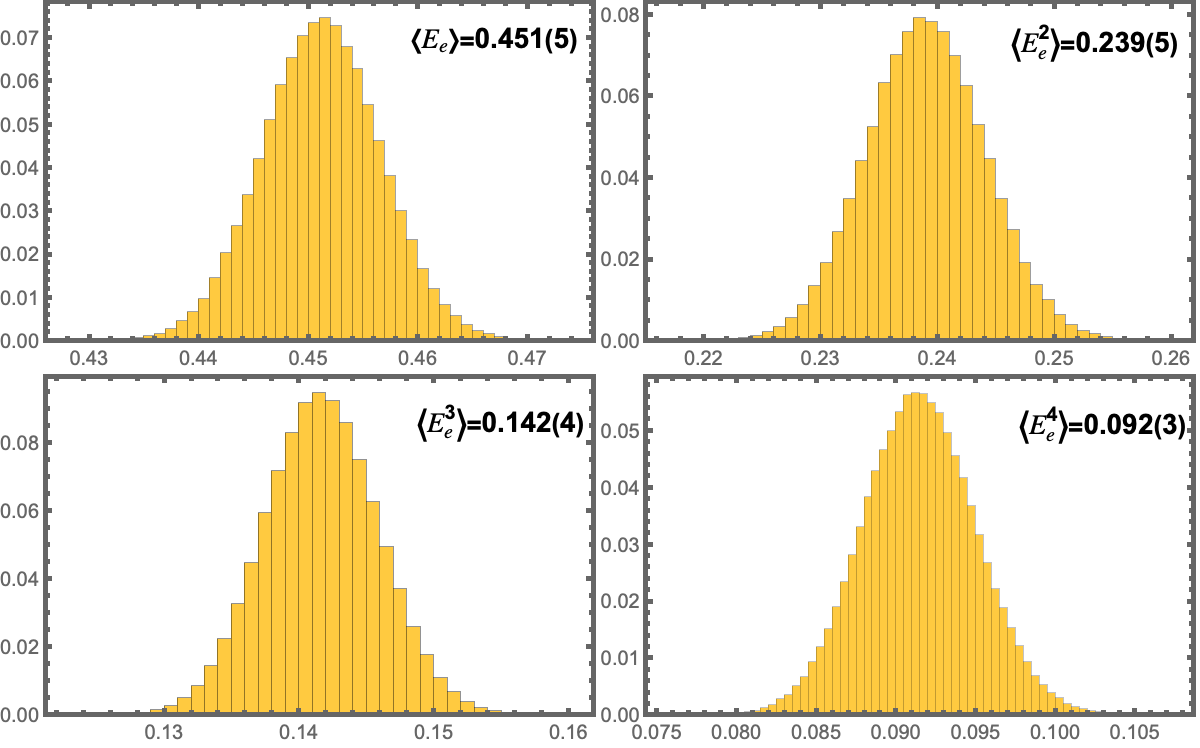
\includegraphics[width=1\textwidth]{figures/H1234.png}
    \caption{实验室系下$\mrm{D\to X e^+\nu_e}$衰变过程的前四阶电子能量矩的概率密度分布}
    \label{fig:Moment_D0_lab}  % 添加标签
\end{figure}

在与电子能量前四阶原点矩的理论表达式进行拟合之前，需通过洛伦兹变换将实验室系下的观测量转换至$\mrm{D_s^+}$质心系。电子能量在$\mrm{D_s^+}$在实验室系与质心系下的关系为：

\begin{equation}
E_{\mathrm{e}}^{\prime} = \gamma E_{\mathrm{e}}(1 - \beta \cos \theta),
\end{equation}
其中，$E_{\mathrm{e}}$ 是电子在 $\mrm{D_s^+}$质心系中的能量，$\beta, \gamma = 1/(\sqrt{1 - \beta^2})$ 是初级顶点上$\mrm{D_s^+}$ 介子的洛伦兹变换因子，$\theta$ 是电子动量在 $\mrm{D_s^+}$ 质心系中的方向与实验室参考系中 $\mrm{D_s^+}$ 介子动量之间的夹角。由于 $\mrm{D_s^+}$ 介子的自旋为零，$\theta$ 的分布是均匀的。可得实验室系下电子能量原点矩和质心系下电子能量原点矩之间的关系为：
\begin{equation}\label{eq:boost}
    \begin{aligned}
     \langle \mrm{E_e} \rangle_{\rm lab} &= \gamma \langle \rm E_e \rangle, & \quad \langle \rm E_e^2 \rangle_{\rm lab} &= \left( 1 + \frac{\beta^2}{3} \right) \gamma^2 \langle\rm E_e^2 \rangle, \\
     \langle \mrm{E_e^3} \rangle_{\rm lab} &= (1 + \beta^2) \gamma^3 \langle \rm E_e^3 \rangle, & \quad \langle \rm E_e^4 \rangle_{\rm lab} &= \left( 1 + 2 \beta^2 + \frac{\beta^4}{5} \right) \gamma^4 \langle \rm E_e^4 \rangle.
    \end{aligned}
  \end{equation}
表\ref{tab:BESIII_Ds_singleyeilds_fit}给出了BESIII合作组实际测量过程中使用的能量点和对应$D_{s}$的估计事例数。$\mrm{e^+ e^-}$对撞产生的$\mrm{D_{s},D^{*}_s}$在实验室系下的动量满足：
\begin{equation}
    \sqrt{p^2 + m_{\mrm{D_s}}^2} + \sqrt{p^2 + m_{\mrm{D_s^{*}}}^2} = E_{\mathrm{cm}},
\end{equation}
其中，$\mrm{D_s^+}$介子的质量为$1.96835\pm 0.00007\GeV$,$D^*_s$介子质量为$2.1122\pm0.0004\GeV$。本文在六个能量点上计算了对应$\mrm{D_s,D^*_s}$的洛伦兹因子$\gamma$,并将每个能量点上$\mrm{D_s^+}$介子的事例数作为权重进行加权求和。最终采用的$\gamma$是$\mrm{D_s^+}$和$\mrm{D_s^*}$介子的算术平均，
\begin{equation}
    \begin{aligned}
        \gamma&=1.02732 \pm 0.00009,\\
        \beta&= 0.2291 \pm 0.0004,\\
    \end{aligned}
    \end{equation}
由于洛伦兹变换因子不确定度较低，因此本文后续的分析将不考虑洛伦兹变换因子的误差。

    至此可得$\mrm{D_s}$静止系的电子能量前四阶矩。应用类似的方法，可得$\mrm{D^0}$,$\mrm{D^+}$介子质心系的电子能量前四阶矩为：
    \begin{equation}
        \scriptsize
        \begin{aligned}
        \left\langle E_e\right\rangle_{\rm exp}^{D_{s}}=0.439(5) \mathrm{GeV}, & \quad\left\langle E_e^2\right\rangle_{\rm exp}^{D_{s}}=0.223(5) \mathrm{GeV}^2, &\left\langle E_e^3\right\rangle_{\rm exp}^{D_{s}}=0.124(4) \mathrm{GeV}^3, &\quad \left\langle E_e^4\right\rangle_{\rm exp}^{D_{s}}=0.074(3) \mathrm{GeV}^4, \\
        \left\langle E_e\right\rangle_{\rm exp}^{D^0}=0.462(5) \mathrm{GeV}, &\quad\left\langle E_e^2\right\rangle_{\rm exp}^{D^0}=0.242(5) \mathrm{GeV}^2,  &\left\langle E_e^3\right\rangle_{\rm exp}^{D^0}=0.138(4) \mathrm{GeV}^3, & \quad\left\langle E_e^4\right\rangle_{\rm exp}^{D^0}=0.084(3) \mathrm{GeV}^4, \\
        \left\langle E_e\right\rangle_{\rm exp}^{D^{+}}=0.455(4) \mathrm{GeV}, & \quad\left\langle E_e^2\right\rangle_{\rm exp}^{D^{+}}=0.236(4) \mathrm{GeV}^2, &\left\langle E_e^3\right\rangle_{\rm exp}^{D^{+}}=0.134(3) \mathrm{GeV}^3, &\quad \left\langle E_e^4\right\rangle_{\rm exp}^{D^{+}}=0.081(3) \mathrm{GeV}^4. \\
        \end{aligned}
        \label{eq:momentRest}
        \end{equation}
    事实上，电子能量原点矩之间存在一定的关联，因此讨论其关联系数并尽可能的降低其关联程度是必要的。
    
    具体而言，本文通过计算皮尔逊积矩系数（Pearson's product-moment coefficient，PPMC）以实现电子能量矩的关联的定量分析。
    \begin{equation}
        \begin{aligned}
            \rho_{X, Y}&=\operatorname{corr}(X, Y)=\frac{\operatorname{cov}(X, Y)}{\sigma_X \sigma_Y}=\frac{\mathrm{E}\left[\left(X-\mu_X\right)\left(Y-\mu_Y\right)\right]}{\sigma_X \sigma_Y}, \quad \text { if } \sigma_X \sigma_Y>0 .\\
            &=\frac{\mathrm{E}(X Y)-\mathrm{E}(X) \mathrm{E}(Y)}{\sqrt{\mathrm{E}\left(X^2\right)-\mathrm{E}(X)^2} \cdot \sqrt{\mathrm{E}\left(Y^2\right)-\mathrm{E}(Y)^2}},
        \end{aligned}
        \end{equation}
        其中，X和Y是任意两组随机变量，\(\operatorname{E}\) 是期望值算符，\(\operatorname{cov}\) 是协方差，\(\operatorname{corr}\) 是PPMC的另一种符号，$\sigma$是随机变量的标准误差，事实上这是柯西-施瓦茨(Cauchy–Schwarz) 不等式的推论，要求即PPMC的绝对值不大于一。因此，相关系数的取值范围在 -1 和 +1 之间。当存在完全正向（递增）线性关系（相关）时，相关系数为 +1；当存在完全反向（递减）线性关系（反相关）时\ct{wearden1991statistics}，相关系数为 -1；在其他情况下，相关系数的值位于开区间 $(-1,1)$ 之间，表示变量之间的线性依赖程度。当相关系数接近零时，表示变量之间的关系较弱（接近无相关性）。相关系数越接近 -1 或 +1，变量之间的相关性越强。

        
    事实上PPMC仅表征两个变量之间的线性依赖程度，PPMC等于零是任意两组随机变量相互独立的必要条件，且无法完全表征两组随机变量之间的关系\ct{anscombe1973graphs}（PPMC是充分统计量的前提是随机变量服从多元正态分布）。
 
    本文讨论了三种D介子的衰变宽度和电子能量原点矩的关联矩阵，为确保准确性，通过散点分布图以实现视觉检查是必要的（$\mrm{D_s^+}$为例）。如图\ref{fig:Moment_Ds_joint}所示，自上（左）到下（右）分别是衰变宽度与电子能量前四阶原点矩。
        \begin{figure}[htbp]
            \centering
            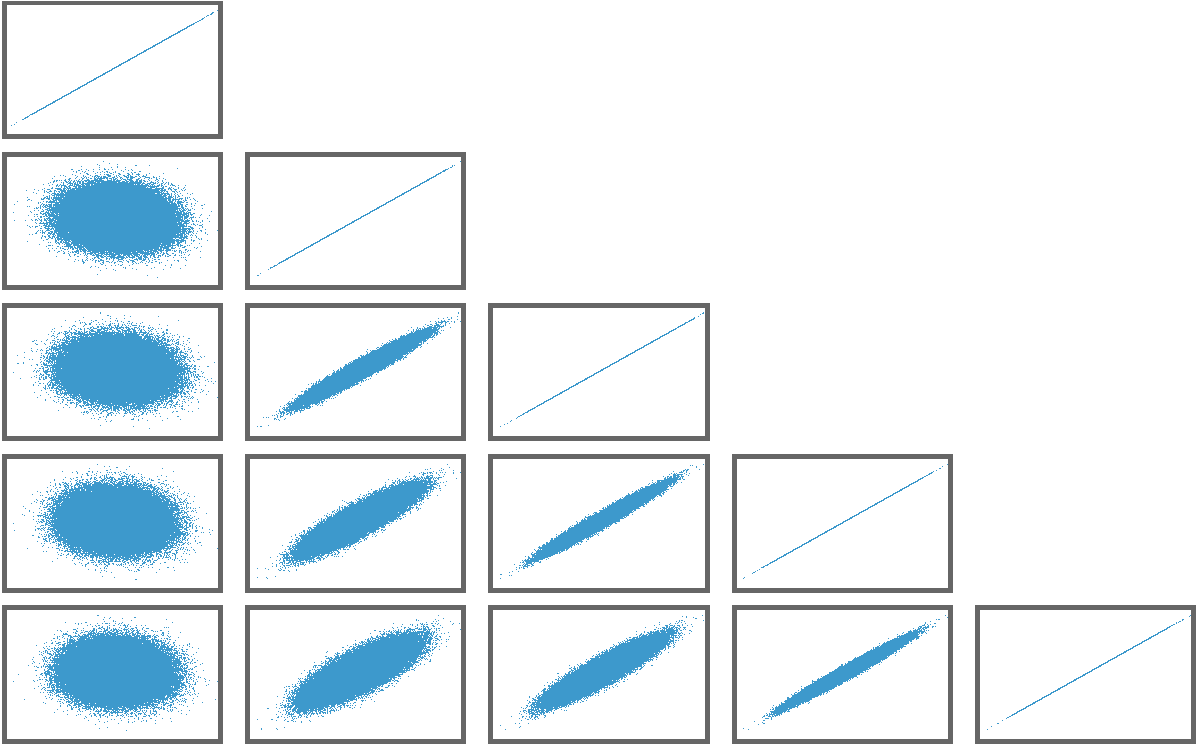
\includegraphics[width=1\textwidth]{figures/jonitsadian.png}
            \caption{$\mrm{D_s^+\to X e^+\nu_e}$衰变过程的衰变宽度与前四阶电子能量原点矩的联合分布}
            \label{fig:Moment_Ds_joint}  % 添加标签
        \end{figure}

        结果表明图\ref{fig:Moment_Ds_joint}与式\eqref{eq:cormoments}的结论保持一致，即衰变宽度与前四阶矩存在微弱负关联且电子能量i阶原点矩与电子能量j阶原点矩关联程度较强。
        \begin{align}\label{eq:cormoments}
            {\rm Cor}(D^0) &= \left(\begin{array}{ccccc}
            1 . & -0.0764818 & -0.0682164 & -0.0584038 & -0.049709 \\
            -0.0764818 & 1 . & 0.964628 & 0.888372 & 0.799743 \\
            -0.0682164 & 0.964628 & 1 . & 0.976053 & 0.921246 \\
            -0.0584038 & 0.888372 & 0.976053 & 1 . & 0.982859 \\
            -0.049709 & 0.799743 & 0.921246 & 0.982859 & 1 .
            \end{array}\right), \nonumber \\
            {\rm Cor}(D^+) &=\left(\begin{array}{ccccc}
            1 . & -0.00918393 & -0.0111696 & -0.011663 & -0.0114986 \\
            -0.00918393 & 1 . & 0.959852 & 0.877876 & 0.784972 \\
            -0.0111696 & 0.959852 & 1 . & 0.974619 & 0.917145 \\
            -0.011663 & 0.877876 & 0.974619 & 1 . & 0.982034 \\
            -0.0114986 & 0.784972 & 0.917145 & 0.982034 & 1 .
            \end{array}\right),\\
            {\rm Cor}(D^+_s) &=\left(\begin{array}{ccccc}
            1 . & -0.0948363 & -0.0854423 & -0.0692735 & -0.0528099 \\
            -0.0948363 & 1 . & 0.961103 & 0.877715 & 0.779303 \\
            -0.0854423 & 0.961103 & 1 . & 0.973193 & 0.910118 \\
            -0.0692735 & 0.877715 & 0.973193 & 1 . & 0.979699 \\
            -0.0528099 & 0.779303 & 0.910118 & 0.979699 & 1 .
            \end{array}\right). \nonumber 
            \end{align}
            
            为了实现对非微扰参数拟合估计的较强约束，降低物理可观测量之间的关联程度是必要的。本文发现存在一组物理可观测量，即$\mrm{D}$介子半轻单举衰变宽度，电子能量一阶原点矩，二三四阶中心矩，其关联程度显著降低。
               电子能量n阶中心矩的定义如下，
                \begin{align}
                    \left\langle \mrm{E_e^n}\right\rangle_{\rm center}\equiv \left\langle (E_e - \langle E_e\rangle)^n \right\rangle,
                    \end{align}
            此外本文也给出了该组物理可观测量的实验抽取结果（表\ref{tab:centermomentRest}）。为了避免该组物理可观测量之间的协方差矩阵出现病态行为\footnote{对某矩阵取逆，出现发散，则称原矩阵为病态矩阵。在计算机数值计算中，由于有限的精度，病态矩阵的逆可能会导致数值结果变得非常大或无穷大（即发散），使得结果没有意义}，需对该组物理可观测量进行重新标度。对应的重标度因子分别是，
            \begin{equation}
                \{10^{15}, 10^3, 10^3, 10^4,10^4\}
                \label{eq:rescaleonTOS}
            \end{equation}
            基于重标度因子可得该组物理可观测量重标度之后的关联矩阵（式\eqref{eq:corcenmoments}），
            \begin{table}[htbp]
                \centering
                \begin{tabular}{lccc}
                    \toprule
                     & \( \mrm{\left\langle E_e^2 \right\rangle_{\text{center}}}/\GeV^2\)  & \(\mrm{ \left\langle E_e^3 \right\rangle_{\text{center}}}/\GeV^3 \) & \(\mrm{ \left\langle E_e^4 \right\rangle_{\text{center}}}/\GeV^4 \)  \\
                    \midrule
                    \(\mrm{ D_s^+} \) & 0.0297(13) & 0.0004(4) & 0.0021(2) \\
                    \( \mrm{D^0} \) & 0.0287(12) & -0.0001(3) & 0.0019(1) \\
                    \(\mrm{D^+} \) & 0.0291(11) & -0.0002(3) & 0.0019(1) \\
                    \bottomrule
                \end{tabular}
                \caption{物理可观测量的实验观测值}
                \label{tab:centermomentRest}
            \end{table}
             \begin{align}\label{eq:corcenmoments}
                {\rm Cor}(D^0) &=\left(\begin{array}{ccccc}
                1 . & -0.0764818 & 0.0281587 & 0.0330765 & 0.0102788 \\
                -0.0764818 & 1 . & -0.088841 & -0.444378 & -0.0618813 \\
                0.0281587 & -0.088841 & 1 . & -0.00420729 & 0.817582 \\
                0.0330765 & -0.444378 & -0.00420729 & 1 . & -0.0351105 \\
                0.0102788 & -0.0618813 & 0.817582 & -0.0351105 & 1 .
                \end{array}\right), \nonumber\\
                {\rm Cor}(D^+) &=\left(\begin{array}{ccccc}
                1 . & -0.00918393 & -0.00799742 & 0.00816853 & -0.0107153 \\
                -0.00918393 & 1 . & -0.0423819 & -0.456701 & -0.0390424 \\
                -0.00799742 & -0.0423819 & 1 . & -0.0538756 & 0.809543 \\
                0.00816853 & -0.456701 & -0.0538756 & 1 . & -0.0924318 \\
                -0.0107153 & -0.0390424 & 0.809543 & -0.0924318 & 1 .
                \end{array}\right), \\
                {\rm Cor}(D^+_s) &=\left(\begin{array}{ccccc}
                1 . & -0.0948363 & 0.0254998 & 0.0800786 & 0.00809594 \\
                -0.0948363 & 1 . & -0.047314 & -0.40486 & -0.0191632 \\
                0.0254998 & -0.047314 & 1 . & 0.0763575 & 0.800281 \\
                0.0800786 & -0.40486 & 0.0763575 & 1 . & 0.172337 \\
                0.00809594 & -0.0191632 & 0.800281 & 0.172337 & 1 .
                \end{array}\right) . \nonumber
                \end{align}
                其中，每一行（列）自左（上）而（下）分别是D介子半轻单举衰变宽度，电子能量一阶矩，电子能量第二、三、阶中心矩。式\eqref{eq:corcenmoments}中的非对角元相比\ref{eq:cormoments}更接近零，这表明新的这组物理可观测量之间的关联强度比使用$\{$衰变宽度，电子能量前四阶原点矩$\}$显著降低。本文以$\mrm{D_s^+}$为对应的该组物理可观测量为例给出联合分布（图\ref{fig:Momentcenter_Ds_joint}）以实现视觉检验。
                \begin{figure}[hbtp]
                    \centering
                    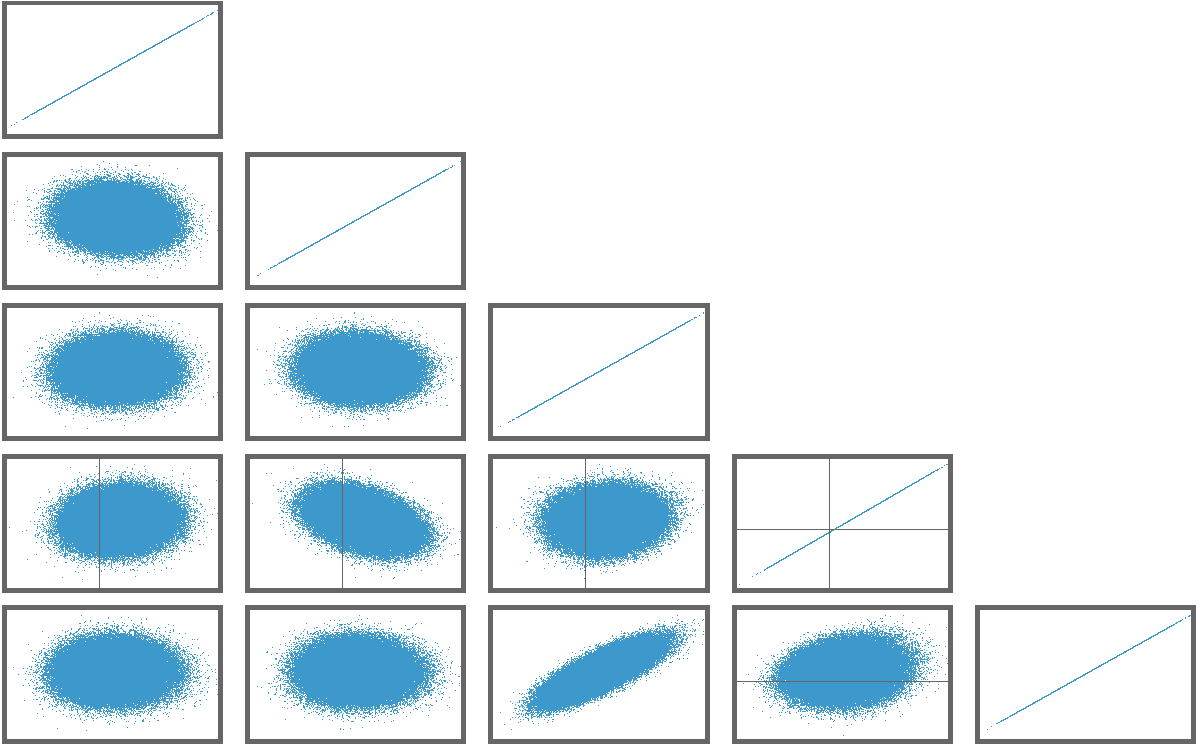
\includegraphics[width=1\textwidth]{figures/jonitsadiancenter.png}
                    \caption{$\mrm{D_s^+\to X e^+\nu_e}$衰变过程的衰变宽度、电子能量一阶原点矩与二、三、四阶中心矩的联合分布}
                    \label{fig:Momentcenter_Ds_joint}  % 添加标签
                \end{figure}

                本节以$\mrm{D_s^+}$为例讨论了电子能量原点矩的抽取，并将其转换到$\mrm{D_s^+}$的质心系;引入PPMC以讨论它们之间的关联强度(式\eqref{eq:cormoments})并与视觉检验（图\ref{fig:Moment_Ds_joint}）形成交叉检验。结果表明：电子能量前四阶原点矩之间存在较强关联，为了对非微扰参数实现更强约束，本文重新抽取了一组物理可观测量：衰变宽度、电子能量一阶原点矩和电子能量第二、三、四阶中心矩。同样地，本文也讨论了它们的关联程度（式\eqref{eq:corcenmoments}和图\ref{fig:Momentcenter_Ds_joint}）。结果表明新的一组物理可观测量之间的关联强度普遍比前者要显著降低，这将有助于对非微扰参数的拟合估计提供更强约束。
                %%%%%%%%%%%%%%%%%%%%%%%%%%%%%%%
\subsection{重夸克质量方案}

第三章在Pole mass scheme下给出了衰变宽度和电子能量前四阶原点矩的理论表达式，并且发现物理可观测量对粲夸克质量高度敏感。事实上用作为重夸克有效理论拉格朗日量参数之一的Pole mass表示的衰变宽度，其高阶微扰修正收敛性非常差。此外不同的charm mass scheme下的粲夸克质量不确定度较低，由于物理可观测量有限，因此本文不对粲夸克质量进行抽取。

由于量子色动力学的夸克禁闭效应导致实验上无法直接测量夸克质量，因此选择适当的质量方案对D介子衰变宽度的理论计算具有关键性的作用。

在壳重整化方案要求在微扰论的每一阶重夸克传播子的逆等于零，对应的重夸克质量称为极质量。尽管极质量作为重夸克有效理论的基本参数之一，但这种质量定义并不是一个好的选择，因为它存在重整化模糊性。这种模糊性表现为极点质量与短程质量的微扰展开级数的收敛性较差，例如在重整化能标$\mu=1.27\GeV$处极质量和$\overline{\mrm{MS}}$质量之间的转换关系为：
\begin{equation}
    \begin{aligned}
    m_\mrm{c}^{\text {Pole }} & =\bar{m}_\mrm{c}\left(\bar{m}_\mrm{c}\right)\left[1+\frac{4}{3} \frac{\alpha_s\left(\bar{m}_c\right)}{\pi}+10.43\left(\frac{\alpha_s\left(\bar{m}_c\right)}{\pi}\right)^2+116.5\left(\frac{\alpha_s\left(\bar{m}_c\right)}{\pi}\right)^3+\cdots\right] \\
    & =\bar{m}_\mrm{c}\left(\bar{m}_\mrm{c}\right)[1+0.1642+0.1582+0.2176+\cdots].
    \end{aligned}
    \end{equation}
    事实上，如果使用$\overline{\mrm{MS}}$质量表示D介子单举衰变宽度，由于重整化能标过于靠近非微扰区域导致其微扰级数的收敛性同样不理想，另一方面，在非常低的尺度下， 
    $\overline{\mrm{MS}}$质量的对数演化是非物理的\ct{Melnikov:2000qh}。为了获得收敛行为良好的微扰展开级数需要合适的粲夸克质量方案。在底强子单举衰变中应用非常成功的质量方案被称为动力学质量方案，其截断能标远离非微扰区域。动力学质量方案和极质量方案之间的关系为\ct{Bigi:1994ga}：
      \begin{equation}
        m_\mrm{Q}^{\text {kin }}(\mu)=m_\mrm{Q}^{\text {Pole }}-[\bar{\Lambda}(\mu)]_{\text {pert }}-\frac{1}{2 m_\mrm{Q}^{\text {kin }}(\mu)}\left[\mu_\pi^2(\mu)\right]_{\text {pert }}+\mathcal{O}\left(\frac{1}{\left(m_\mrm{Q}^{\text {kin }}\right)^2}\right),
        \end{equation}
    其中Q是重夸克,$\bar{\Lambda}$ 和 $\mu_\pi^2$的领头阶的表达式为\ct{Bigi:1994ga}：
        \begin{equation}
            \begin{aligned}
            & {[\bar{\Lambda}(\mu)]_{\mathrm{pert}}=\frac{16}{9} \frac{\alpha_s}{\pi} \mu+\mathcal{O}\left(\alpha_s^2\right)}, \\
            & {\left[\mu_\pi^2(\mu)\right]_{\mathrm{pert}}=\frac{4}{3} \frac{\alpha_s}{\pi} \mu^2+\mathcal{O}\left(\alpha_s^2\right)},
            \end{aligned}
            \end{equation}
    $\mu$是截断能标。在动力学质量方案下，极质量中的微扰级数被$[\bar{\Lambda}(\mu)]_{\text {pert }}$ 和 $\left[\mu_\pi^2(\mu)\right]_{\text {pert }}$修改。此外，重夸克有效理论中的参数也将被重新定义\ct{Gambino:2007rp, Gambino:2017vkx}，
    \begin{equation}
        \begin{aligned}
        \mu_\pi^2 & =\mu_\pi^{2, \mathrm{kin}}+\left[\mu_\pi^2(\mu)\right]_{\mathrm{pert}}=\mu_\pi^{2, \mathrm{kin}}+\frac{4}{3} \frac{\alpha_s}{\pi} \mu^2, \\
        \rho_D^3 & =\rho_D^{3, \mathrm{kin}}+\left[\rho_D^3(\mu)\right]_{\mathrm{pert}}=\rho_D^{3, \mathrm{kin}}+\frac{8}{9} \frac{\alpha_s}{\pi} \mu^3.
        \end{aligned}
        \end{equation}
        重夸克有效理论中$\mrm{(\Lambda_{QCD}/m_{Q})^{n}}$的项产生了 $\mrm{\left(\frac{\alpha_s}{\pi}\right) \frac{\mu^n}{m_Q^n}}$ 阶的修正，这使得截断尺度的选择窗口很小。一方面，它必须比重夸克质量小，使得 $\frac{\mu}{m_\mrm{Q}}$ 是一个收敛行为良好的展开参数；另一方面，它应该处于微扰区域。截断能标在$\mu= 1\GeV$的动力学质量方案已成功应用于B介子单举衰变（参见例如\ct{Alberti:2014yda,Gambino:2016jkc}）。

        对于本文研究的粲介子单举衰变若存在类似的动力学质量方案，则其截断能标$\mu$的选择窗口显著降低。

        本文采用的质量方案之一是$\overline{\mrm{MS}}$质量方案，并在两圈图水平上将其转换为极质量\ct{Chetyrkin:2000yt}，如式\eqref{eq:MSbar}所示，
        \begin{equation}
            \begin{aligned}
                m_{\text{c}}^{\text{pole}} = m_{\text{c}} &+ m_{\text{c}}\frac{\left(\frac{4}{3} + \log \left[\frac{\mu^2}{m_{\text{c}}^2}\right]\right) \alpha_s}{\pi} \\
                &+m_{\text{c}} \frac{\alpha_s^2\left(\frac{779}{96} + \frac{\pi^2}{6} + \frac{1}{9} \pi^2 \log [2] + \frac{415}{72} \log \left[\frac{\mu^2}{m_{\text{c}}^2}\right] + \frac{37}{24} \log \left[\frac{\mu^2}{m_{\text{c}}^2}\right]^2 - \frac{\zeta(3)}{6}\right)}{\pi^2},
            \end{aligned}
                \label{eq:MSbar}
            \end{equation}

        其中，$m_{\mrm{c}}$是$\mrm{\overline{MS}}$质量方案下的粲夸克质量，$m_{\mrm{c}}^{\text{pole}}$是极质量方案下的粲夸克质量，$\mu$是重整化能标。
        
        本文采用的另外一个质量方案是1S质量方案，1S质量主要应用于夸克的束缚态质量，如底夸克和粲夸克，尤其是在强相互作用下产生的夸克对中，比如$\Upsilon$和$J/\psi$这样的$q\bar{q}$束缚态。文献\ct{Hoang:1998ng}给出了两圈图水平上1S质量和极质量之间的转换关系。对其取逆并展开到$\epsilon^2$阶，得到极质量与1S质量之间的转换关系，如式\eqref{eq:1S}所示,
        \begin{equation}
            m_\mrm{c}^{\text{Pole}}=m_\mrm{c}+\frac{2}{9} m_\mrm{c}\epsilon \alpha_s^2-\frac{\epsilon^2 m_\mrm{c}\left(-\frac{12992 \alpha_s^3}{9}-\frac{3200}{3} \log \left[\frac{3 \mu}{4 m_\mrm{c} \alpha_s}\right] \alpha_s^3-\frac{256 \pi \alpha_s^4}{9}\right)}{576\pi},
            \label{eq:1S}
        \end{equation}
        其中，$m\mrm{c}$是1S质量方案下的粲夸克质量，$\epsilon$是1S质量方案下的展开参数，$\epsilon$的线性项表示单圈水平，平方项表示两圈图水平。取$J/\psi$质量的1/2作为粲夸克的1S质量，即$m_{\mrm{c}}=1.55\GeV$。
        此外本文计算了1S质量方案下$\mrm{D}$介子半轻单举衰变宽度的微扰展开级数为
        \begin{equation}
            \Gamma_{\mrm{sl}}^{\mrm{D}}\sim 1-0.131-0.048+0.019+\cdots,
        \end{equation}
        从左至右分别是领头阶(Leading Order, LO)，次领头阶(Next to leading Order, NLO)，次次领头阶(Next Next to leading Order, NNLO)和次次次领头阶（Next Next Next to leading Order, NNNLO）的修正($\mrm{\alpha_s=0.387}$)。极质量方案下D介子半轻单举衰变宽度的微扰展开级数为
        $$\Gamma_{\mrm{sl}}^{\mrm{D}}\sim1-0.768104 \alpha_s-2.37521 \alpha_s^2-10.7295 \alpha_s^3+\cdots,$$
        收敛行为较差。因此，1S质量方案是比较合适的粲夸克质量方案，本文的唯象学分析将讨论$\overline{\text{MS}}$和1S质量方案下的全局拟合。
\subsection{唯象学分析}
为从$\mrm{D}$介子半轻单举衰变的实验数据中实现重夸克有效理论非微扰参数的拟合估计。本文采用$\mrm{D\to X_{\rm{c},\rm{s}} e^+ \nu_{e}}$过程的衰变宽度，电子能量一阶原点矩与电子能量第二、三、四阶中心矩的实验观测值和相应理论表达式进行全局拟合。在幂次修正精确至量纲六算符的精度下，包含以下的微扰参数：
\begin{equation}
    \begin{aligned}
        &\mu_{\pi}^2(\mrm{D^{0,+}}),\quad \mu_{\mrm{G}}^{2}(\mrm{D^{0,+}}),\quad \rho_{\mrm{D}}^3(\mrm{D^{0,+}}),\quad \rho_{\mrm{LS}}^3(\mrm{D^{0,+}}), \\
        &\mu_{\pi}^2(\mrm{D_s^+}),\quad\;\:\; \mu_{\mrm{G}}^{2}(D_s^+),\quad\;\:\: \rho_{\mrm{D}}^3(D_s^+),\quad\;\:\; \rho_{\mrm{LS}}^3(\mrm{D_s^+}),
    \end{aligned}
    \end{equation}
    
    
    
    

其中，由于同位旋对称性的约束，对$\mrm{D^{0}}$和$\mrm{D^{+}}$的非微扰参数不作区分。这些非微扰参数在粲介子寿命的理论计算，粲介子稀有衰变，甚至底介子的单举衰变中扮演了举重若轻的角色。量纲六算符也包含四夸克算符，基于真空插入近似\ct{Bauer:1986bm}（Vacuum Insertion Approximation， VIA）,四夸克算符非微扰矩阵元矩阵元对衰变宽度的贡献可以忽略不计。

为了讨论幂次展开的收敛性对拟合抽取重夸克有效理论中非微扰参数的影响，我们将在两种情形下进行全局拟合。对于情形$\mrm{I}$，物理可观测量的理论表达式的幂次修正仅精确至量纲五算符的贡献；对于情形$\mrm{II}$, 物理可观测量的理论表达式的幂次修正仅精确至量纲六算符的贡献。此外基于上节的讨论，本节将讨论三种不同的质量方案下非微扰参数的拟合估计。

由于重整化能标$\mu$的跑动会引起强相互作用耦合常数的浮动，因此讨论理论输入参数的误差对拟合估计非微扰参数的影响是必要的，经过对所有理论输入参数的误差评估，最终仅引入由于重整化能标的跑动导致强相互作用耦合常数的浮动误差。具体地，首先固定相关的理论输入参数并进行相关的全局拟合估计，对应非微扰参数的估计值作为非微扰参数的拟合估计中心值，对应非微扰参数的估计误差作为非微扰参数误差的实验部分；其次，使用MC技术完成2000次的相关拟合，取相关拟合关于非微扰参数的估计值分布的标准误差作为非微扰参数误差的理论部分。本文粗略地假设非微扰参数误差的理论部分和实验部分相互独立，基于误差传递公式得到非微扰参数的拟合估计误差。

在拟合过程中，本文使用了奇异夸克质量的 $2+1+1$ 格点 QCD FLAG 平均值，$\overline{m}_s(2 \mathrm{GeV}) = 93.44$ MeV~\cite{FlavourLatticeAveragingGroup:2019iem}。对于粲夸克质量，本文使用 $m_{c}^{\overline{\mrm{MS}}} = 1.27$ GeV 和 $m_{c,\mathrm{1S}} = 1.55$ GeV~\cite{ParticleDataGroup:2024cfk}。对于强耦合常数，本文采用Lenz等人在~\cite{King:2021xqp} 中通过 RunDec 包~\cite{Herren:2017osy} 获得的强相互作用耦合常数 $\alpha_{s}(\ov{m}_{c}) = 0.387$。对于 $\alpha_s(\mu)$ 和 $\ov{m}_c(\mu)$，本文考虑了从 1 GeV 到 $2\ov{m}_{c}(\ov{m}_{c})$ 的跑动 $\mu$。此外使用以下输入值用于理论公式中的其他参数~\cite{ParticleDataGroup:2024cfk}，$\mrm{G_F} = 1.1663788 \times 10^{-5}$，$\mrm{|V_{cs}|} = 0.975$，以及 $\mrm{|V_{cd}|} = 0.221$.

\subsubsection{一. 固定理论输入参数}
基于本文第三章理论部分的研究，可得到了三种D介子在极质量方案下的的衰变宽度，电子能量一阶原点矩与电子能量第二、三、四阶中心矩的理论表达式。此外本文提供了$\overline{\mrm{MS}}$ 和$\mrm{1S}$质量方案下物理可观测量微扰修正部分的理论表达式（附录\ref{app:TOS}）

定义物理可观测量的理论表达式\footnote{在实际全局拟合过程中，需要对$\aleph$的每个元素乘以式\eqref{eq:rescaleonTOS}相对应的标度因子}是集合$\aleph$，
\begin{equation}
    \begin{aligned}
        \aleph_{theory}^{D^{0}} := & \{\Gamma^{D^{0,+}}, \langle E_{e}\rangle^{D^{0,+}}, \langle E_{e}^2\rangle^{D^{0,+}}_{\text{center}}, \langle E_{e}^3\rangle^{D^{0,+}}_{\text{center}}, \langle E_{e}^4\rangle^{D^{0,+}}_{\text{center}}\}, \\
        \aleph_{theory}^{D^{+}} := & \{\Gamma^{D^{0,+}}, \langle E_{e}\rangle^{D^{0,+}}, \langle E_{e}^2\rangle^{D^{0,+}}_{\text{center}}, \langle E_{e}^3\rangle^{D^{0,+}}_{\text{center}}, \langle E_{e}^4\rangle^{D^{0,+}}_{\text{center}}\}, \\
        \aleph_{theory}^{D_s} := & \{\Gamma^{D_{s}},\langle E_{e}\rangle^{D_{s}}, \langle E_{e}^2\rangle^{D_{s}}_{\text{center}}, \langle E_{e}^3\rangle^{D_{s}}_{\text{center}}, \langle E_{e}^4\rangle^{D_{s}}_{\text{center}}\}.
    \end{aligned}
    \label{eq:TOS}
\end{equation}
重标度后对应的物理可观测量的实验观测值为：
\begin{equation}
    \begin{aligned}
        \aleph_{\text{exp, rescaled}}^{D^0} &:= \{102.137,461.653,28.7391,-1.10121,19.1876\}, \\
        \aleph_{\text{exp, rescaled}}^{D^+} &:=\{102.192,455.073,29.0727,-2.36531,19.7269\},\\
        \aleph_{\text{exp, rescaled}}^{D_s} &:=\{82.9754,439.393,29.6515,3.43014,21.3503\},\\
        \sigma(\aleph_{\text{exp, rescaled}}^{D^0})&:=\{2.40402,4.92835,1.21868,3.36424,1.33466\},\\
        \sigma(\aleph_{\text{exp, rescaled}}^{D^+})&:=\{2.03942,4.23467,1.1135,3.1932,1.22891\},\\
        \sigma(\aleph_{\text{exp, rescaled}}^{D_s})&:=\{1.98213,5.18726,1.29376,3.90018,1.6387\},\\
    \end{aligned}
    \label{eq:expdata}
\end{equation}
前三行是这组物理可观测量$\aleph$的中心值，后三行是这组物理可观测量$\aleph$的标准误差。

一般地，在 $n$ 个观测点通过测量得到一组 $n$ 个观测值 $\boldsymbol{y}=$ $\left(y_1, y_2, \cdots, y_n\right)^{\mathrm{T}}$ ，相应的观测值真值 $\boldsymbol{\eta}=\left(\eta_1, \eta_2, \cdots, \eta_n\right)^{\mathrm{T}}$ 为末知，它由某个理论
模型预期：$\eta_i=f\left(x_i, \boldsymbol{\theta}\right)(i=1,2, \cdots, n)$ ，其中 $\boldsymbol{\theta}=\left(\theta_1, \theta_2, \cdots, \theta_k\right)^{\mathrm{T}}$ 是待定的参数． $\theta$ 的最小二乘估计可由最小二乘函数 $Q^2(\boldsymbol{\theta})$ 的极小值求得
\begin{equation}
    Q^2(\boldsymbol{\theta})=(\boldsymbol{y}-\boldsymbol{\eta}(\boldsymbol{\theta}))^{\mathrm{T}} \boldsymbol{V}^{-1}(\boldsymbol{y}-\boldsymbol{\eta}(\boldsymbol{\theta}))=\sum_{i=1}^n \sum_{j=1}^n\left(y_i-\eta_i\right) V_{i j}^{-1}\left(y_j-\eta_j\right),
    \end{equation}
其中，$\boldsymbol{\theta}$是某个理论所包含的参数，$V$是测量值之间的协方差矩阵，若这组观测量之间相互独立，则$ Q^2(\boldsymbol{\theta})$约化为：$$
Q^2(\boldsymbol{\theta})=\sum_{i=1}^n\left(\frac{y_i-\eta_i}{\sigma_i}\right)^2,
$$
其中，$\sigma_{i}$是第i个测量值的标准误差。
定义最小二乘函数构造如下\footnote{l=u,d,s分别对应于$\mrm{D^{0}}, \mrm{D^{+}},\mrm{D_s^+}$}，
\begin{equation}
    \begin{aligned}
        Q^2(\boldsymbol{\theta})=&\sum_{l=u,d,s}\sum_{i=1}^{5}\sum_{j=1}^{5}\times\\
        &(\aleph_{\text{exp, rescaled}, i}^{D^l}-\aleph_{\text{theory, rescaled, i}}^{D^l})V_{i j,l}^{-1}(\aleph_{\text{exp, rescaled} ,j}^{D^l}-\aleph_{\text{theory, rescaled, j}}^{D^l})^{\text{T}},\\
    \end{aligned}
    \label{eq:chi2_func}
\end{equation}
其中$V_{ij,l}$是$\mrm{D^{l}}$介子五组数据之间的协方差矩阵。基于Mathematica进行非微扰参数的全局拟合估计，采用 DifferentialEvolution, SimulatedAnnealing, RandomSearchd等算法对搜索到的全局最小点进行交叉检验。此外本文基于Python完成了固定理论输入参数的前提下两种情形的全局拟合估计作为进一步交叉检验。
\paragraph{极质量方案}
我们选取两圈图水平上的极质量，即$m_{\mrm{c}}=1.67\GeV$.
拟合结果表明，对于情形$\mrm{I}$, $\chi^{2}_{\text{min}}=195.522$, $\chi^{2}_{\text{min}}/\text{d.o.f}=17.77$
\begin{equation}
    \mu_{\pi}^2(\mrm{D^{0,+}})\to 0.05,\;\mu_{\mrm{G}}^{2}(\mrm{D^{0,+}})\to -0.02, \;\mu_{\pi}^2(\mrm{D_s^+})\to 0.06, \;\mu_{\mrm{G}}^{2}(\mrm{D_s^+})\to 0.08
\end{equation}
对于情形$\mrm{II}$, $\chi^{2}_{\text{min}}=26.24$, $\chi^{2}_{\text{min}}/\text{d.o.f}=3.74$
\begin{equation}
    \begin{aligned}
        &\mu_{\pi}^2(\mrm{D^{0,+}})\to 0.11,\;\mu_{\mrm{G}}^{2}(\mrm{D^{0,+}})\to -0.03, \;\mu_{\pi}^2(\mrm{D_s^+})\to 0.15, \;\mu_{\mrm{G}}^{2}(\mrm{D_s^+})\to 0.08\\
        &\rho_{\mrm{D}}^3(\mrm{D^{0,+}})\to -0.005,\;\rho_{\mrm{LS}}^3(\mrm{D^{0,+}})\to 0.006, \;\rho_{\mrm{D}}^3(\mrm{D_s^+})\to -0.007, \;\rho_{\mrm{LS}}^3(\mrm{D_s^+})\to 0.007
    \end{aligned}
\end{equation}
极质量方案下D介子半轻单举衰变宽度的高阶微扰修正和幂次修正的收敛性较差，下面仅讨论$\overline{\mrm{MS}}$质量方案和$\mrm{1S}$质量方案下的拟合估计结果和相应误差分析。
\paragraph{$\overline{\mrm{MS}}$质量方案}
上一节我们讨论了两圈图水平上$\overline{\mrm{MS}}$质量和极质量之间的转换关系（式\eqref{eq:MSbar}）。将$\aleph_{\text{theory}}$中的物理可观测量在两圈图水平上用$\overline{\mrm{MS}}$质量表示出来(其微扰部分的具体形式见附录\ref{app:TOS}), 重整化能标取在粲夸克$\overline{\mrm{MS}}$质量处，即$\mu=1.27\GeV$,全局拟合估计结果如表\ref{tab:MS_fitting}所示
\begin{table}[h!]
    \scriptsize
    \begin{tabular}{cllllll} % 使用 | 添加竖线
    \hline
      $\mathrm{\overline{MS}}$ 方案&$\chi^2_{\text{tot}}$&$\mrm{D_{i}}$&$\mrm{\mu_{\pi}^{2}}$/$\mathrm{GeV^2}$&$\mrm{\mu_{G}^{2}}$/$\mathrm{GeV^2}$&$\mathrm{\rho_{D}^{3}}$/$\mathrm{GeV^3}$ &$\mrm{\rho_{LS}^{3}}$/$\mathrm{GeV^3}$ \\ % 表格内容
      \hline
     \multirow{2}{*}{\text{情形I}} & \multirow{2}{*}{\scriptsize{49.26}}  & $\mrm{D^{0,+}}$&\scriptsize{$0.09\pm0.01\pm.$}&\scriptsize{$0.27\pm 0.01\pm0.14$}&-&-\\
     &&$\mrm{D_s^+}$&\scriptsize{$0.09\pm 0.01\pm$0.01}&\scriptsize{$0.39\pm 0.01\pm 0.12$}&-&-\\
      \hline
      \multirow{2}{*}{\text{情形II}}  &  \multirow{2}{*}{\scriptsize{14.53}}  & $\mrm{D^{0,+}}$ &\scriptsize{$0.11\pm0.01\pm0.02$}&\scriptsize{$0.26\pm 0.01\pm0.14$}&\scriptsize{$-0.002\pm 0.001\pm0.001$}&\scriptsize{$0.003\pm 0.001\pm0.001$}\\
      &&$\mrm{D_s^+}$&\scriptsize{$0.12\pm0.01\pm0.02$}&\scriptsize{$0.38\pm0.01\pm0.13$}&\scriptsize{$-0.003\pm0.001\pm 0.001$}&\scriptsize{$0.005\pm 0.001\pm0.001$}\\  \hline
    \end{tabular}
    \caption{$\overline{\mrm{MS}}$质量方案下对非微扰参数的全局拟合估计结果}
    \label{tab:MS_fitting}
    \end{table}
    表\ref{tab:MS_fitting}中的第一个误差来源于实验，第二个误差来源于强相互作用耦合常数跑动带来的理论误差。情形$\mrm{I}$和$\mrm{II}$关于非微扰参数的拟合估计值非常接近，这反映了幂次修正的收敛行为较好。
\paragraph{$\mrm{1S}$质量方案}两圈图水平上1S质量和极质量之间的转换关系及其对重整化能标的具体依赖形式（式\eqref{eq:1S}），将$\aleph_{\text{theory}}$中的物理可观测量在两圈图水平上用$\mrm{1S}$质量表示出来(其微扰部分的具体形式见附录\ref{app:TOS}), 重整化能标取在粲夸克$\overline{\mrm{MS}}$质量处，即$\mu=1.27\GeV$,全局拟合结果如表\ref{tab_1S_fitting}所示,
\begin{table}[h!]
    \scriptsize
    \begin{tabular}{cllllll} % 使用 | 添加竖线
    \hline
     1S 质量方案&$\chi^2_{\text{tot}}$&$\mrm{D_{i}}$&$\mu_{\pi}^{2}$/$\mathrm{GeV^2}$&$\mu_{\mrm{G}}^{2}$/$\mathrm{GeV^2}$&$\mathrm{\rho_{\mrm{D}}^{3}}$/$\mathrm{GeV^3}$ &$\rho_{\mrm{LS}}^{3}$/$\mathrm{GeV^3}$ \\ % 表格内容
      \hline
     \multirow{2}{*}{\text{情形} I} & \multirow{2}{*}{\scriptsize{54.06}}  & $\mrm{D^{0,+}}$&\scriptsize{$0.04\pm0.003\pm0.010$}&\scriptsize{$0.33\pm 0.01\pm0.01$}&-&-\\
     &&$\mrm{D_s^+}$&\scriptsize{$0.06\pm 0.01\pm 0.01$}&\scriptsize{$0.44\pm 0.01\pm 0.02$}&-&-\\
      \hline
      \multirow{2}{*}{\text{情形} II}  &  \multirow{2}{*}{\scriptsize{$2.32$}}  & $\mrm{D^{0,+}}$&\scriptsize{$0.09\pm0.01\pm 0.01$}&\scriptsize{$0.32\pm0.01\pm0.01$}&\scriptsize{$-0.003\pm0.001\pm0.001$}&\scriptsize{$0.004\pm 0.001\pm0.001$} \\
      &&$\mrm{D_s^+}$&\scriptsize{$0.11\pm0.01\pm0.01$}&\scriptsize{$0.43\pm 0.01\pm0.02$}&\scriptsize{$-0.004\pm 0.001\pm0.001$}&\scriptsize{$0.005\pm0.001\pm0.001$}\\  \hline
    \end{tabular}
    \caption{1S质量方案下对非微扰参数的全局拟合结果}
    \label{tab_1S_fitting}
    \end{table}
    表\ref{tab_1S_fitting}中的第一个误差来源于实验，第二个误差来源于强相互作用作用耦合常数跑动引入的误差。1S 质量方案情形$\mrm{II}$的平均最小卡方值小于一，即在这种情形下具有良好的拟合效果；此外1S质量方案下幂次修正对非微扰参数的估计值影响同样较弱。


    %%%%%%%%%%%%%%%%%%%%%%%%%%%%%%%%%%%%%%
    此外本文计算了1S质量方案下情形$\mrm{II}$中非微扰参数拟合估计的关联矩阵（式\eqref{eq:corpara}），
    \begin{align}\label{eq:corpara}
        {\rm Cor}(D^{0,+})&=
        \left(\begin{array}{cccc}
        1 . & -0.247711 & -0.920525 & 0.85145 \\
        -0.247711 & 1 . & 0.325483 & -0.325445 \\
        -0.920525 & 0.325483 & 1 . & -0.971566 \\
        0.85145 & -0.325445 & -0.971566 & 1 .
        \end{array}\right), \\
        {\rm Cor}(D_{s}^+)&=
        \left(\begin{array}{cccc}
        1 . & -0.256407 & -0.901138 & 0.842813 \\
        -0.256407 & 1 . & 0.324073 & -0.32296 \\
        -0.901138 & 0.324073 & 1 . & -0.97023 \\
        0.842813 & -0.32296 & -0.97023 & 1 .
        \end{array}\right), \nonumber
        \end{align}
        式\eqref{eq:corpara}自上（左）而（右），分别是$\mu_{\pi}^{2}$, $\mu_{\mrm{G}}^{2}$, $\rho_{\mrm{D}}^{3}$,和$\rho_{\mrm{LS}}^3$。
    情形$\mrm{II}$相比于情形$\mrm{I}$而言，由于引入了量纲六算符的微扰参数使得最小卡方值迅速降低，表明量纲六算符的非微扰矩阵元的贡献在物理可观测量计算中具有举足轻重的作用，且此现象的存在与否并不依赖于粲夸克质量方案。这一事实确信了量纲六算符修正对物理可观测量的理论预言非常重要。由于物理可观测量有限，暂时无法实现对量纲六算符中四夸克算符的非微扰矩阵元的拟合估计。期待未来构建足够多的物理可观测量得以进行更丰富的全局拟合估计，从而确定高量纲算符的非微扰矩阵元。这样的工作无论是对于重夸克有效理论在粲强子弱衰变的典型能标处的发展还是对于粲强子的寿命疑难的理解甚至解决均有重要的意义。
\subsubsection{二. 引入理论输入参数的误差}
上一节在固定所有理论输入参数的前提下进行全局拟合估计。事实上，理论输入参数的误差对非微扰参数的拟合估计具有不可忽视的影响。在评估所有理论输入参数的误差相对大小之后，本文舍弃次要矛盾抓住主要矛盾，仅考虑由于重整化能标的跑动引起强相互作用耦合常数跑动。本节主要讨论重整化能标$\mu$和强相互作用耦合常数$\alpha_s(\mu)$所带来的理论误差\footnote{其余部分的误差与其相比基本忽略不计}。

强相互作用耦合常数满足重整化群方程(式\eqref{eq:alphas_eq_QCD})，
\begin{equation}
    \mu_R^2 \frac{d \alpha_s}{d \mu_R^2}=\beta\left(\alpha_s\right)=-\left(\beta_0 \alpha_s^2+\beta_1 \alpha_s^3+\beta_2 \alpha_s^4+\beta_3 \alpha_s^5\cdots\right).
    \label{eq:alphas_eq_QCD}
    \end{equation}
式\eqref{eq:alphas_eq_QCD}中，  \( \beta_0 = (11 C_A - 4 n_f T_R)/(12 \pi) = (33 - 2 n_f)/（12 \pi） \) 被称为 单圈\(\beta\)函数系数，两圈系数为 \( \beta_1 = (17 C_A^2 - n_f T_R (10 C_A + 6 C_F))/（24 \pi^2） = (153 - 19 n_f)/（24 \pi^2） \)，三圈系数为 \( \beta_2 = (2857 - 5033/9 n_f + 325/27 n_f^2)/（128 \pi^3）\), \( C_A =3\) 和 \( C_F=4/3 \), \( n_f \) 是具体过程涉及夸克味道数。

对于仅考虑$n_{f}$种夸克的相互作用且其重整化能标$\mu_{R}$处的有效理论对应的强相互作用耦合常数对夸克数$n_{f}$存在依赖。一般地，对于涉及$n_{f}$和$n_{f}+1$种味道的强相互作用耦合常数之间存在一种迭代关系，
\begin{equation}
    \alpha_s^{\left(n_f+1\right)}\left(\mu_R^2\right)=\alpha_s^{\left(n_f\right)}\left(\mu_R^2\right)\left(1+\sum_{n=1}^{\infty} \sum_{\ell=0}^n c_{n \ell}\left[\alpha_s^{\left(n_f\right)}\left(\mu_R^2\right)\right]^n \ln ^{\ell} \frac{\mu_R^2}{m_h^2}\right).
    \label{eq:alpha_s_replace}
    \end{equation}
其中 \(m_h\) 是第 \(\left(n_f+1\right)\) 味的夸克质量， \(c_{11}=1/(6 \pi), c_{10}=0\)，\(c_{22}=c_{11}^2, c_{21}=11/(24 \pi^2)\)， \(c_{20}=-11/(72 \pi^2)\)， \(m_h\) 是在 \(m_h\) 处的 \(\mrm{\overline{\text{MS}}}\) 质量.此外，对式\eqref{eq:alphas_eq_QCD}进行迭代求解，存在一个近似解析解，
\begin{equation}
\scriptsize
\alpha_s\left(\mu_R^2\right)  \simeq \frac{1}{\beta_0 t}\left(1-\frac{\beta_1 \ell}{\beta_0^2} \frac{1}{t}+\frac{\beta_1^2\left(\ell^2-\ell-1\right)+\beta_0 \beta_2}{\beta_0^4 t^2} 
+\frac{\beta_1^3\left(-2 \ell^3+5 \ell^2+4 \ell-1\right)-6 \beta_0 \beta_2 \beta_1 \ell+\beta_0^2 \beta_3}{2 \beta_0^6 t^3}\right)+\cdots.
\label{eq:alpha_s_solution}
\end{equation}
存在两种方式可得粲介子半轻单举衰变典型能标处的强相互作用耦合常数的解析形式: 
\begin{itemize}
\item 使用$\mu=m_{z}$处的$\alpha_s$，利用式\eqref{eq:alpha_s_replace}进行迭代求解，最终迭代至目标能标处。
\item 若衰变的典型能标出的$\alpha_s$已知，可以使用式\eqref{eq:alpha_s_solution}在典型能标处求解出$\Lambda_{n_{f}}$,重新带入式\eqref{eq:alpha_s_solution}得到典型衰变能标附近$\alpha_s$关于重整化能标$\mu$的具体依赖形式。
\end{itemize}
Alexander Lenz等人于2022年重新计算了D介子的寿命\ct{King:2021xqp},他们给出并采用五圈图水平上$\alpha_s(\mu=1.27\GeV)$的数值结果，$\alpha_s(\mu=1.27\GeV)=0.387$.本文以该值为基准，按照方式二($\mrm{n_{f}=4}$)计算可得重整化能标$\mu=1.27\GeV$处$\alpha_s$关于$\mu$的具体依赖形式。

具体而言，本文引入由重整化能标$\mu$的跑动带来$\alpha_s$的误差，其中重整化能标$\mu$被假设服从$[1, 2.54]\GeV$的Uniform Distribution。利用MC模拟，本文给出了2000个重整化能标$\mu$的样本，结合强相互作用对重整化能标的具体依赖形式可得一组强相互作用耦合常数，并完成2000次$\chi^{2}$拟合。

拟合结果如表\ref{tab:MS_fitting}和\ref{tab_1S_fitting}所示。在讨论理论输入参数误差对非微扰参数的拟合估计影响基础上，本文进一步讨论了幂次修正对非微扰参数拟合估计的影响。

由于1S 质量方案下衰变宽度的微扰修正和幂次修正收敛性较好，因此本文采取1S质量方案下的拟合结果作为本文关于非微扰参数的推荐值，如式\eqref{fitting}所示。
\begin{equation}
\begin{aligned}
    \mu^2_\pi(\mrm{D^{0,+}}) &= (0.09\pm 0.05) \mathrm{GeV}^2, \qquad \qquad
    \mu^2_\pi(\mrm{D^{+}_s}) = (0.11\pm 0.05) \mathrm{GeV}^2,  \\
    \mu^2_\mrm{G}(\mrm{D^{0,+}}) &= (0.32\pm 0.02) \mathrm{GeV}^2, \qquad \qquad 
    \mu^2_\mrm{G}(\mrm{D^{+}_s}) = (0.43\pm 0.02) \mathrm{GeV}^2, \nonumber \\
    \rho_\mrm{D^3}(\mrm{D^{0,+}}) &= (-0.003\pm 0.002) \mathrm{GeV}^3, \qquad\ 
    \rho_\mrm{D^3}(\mrm{D^{+}_s}) = (-0.004\pm 0.002) \mathrm{GeV}^3, \nonumber \\
    \rho_{LS}^3(\mrm{D^{0,+}}) &= (0.004\pm 0.002) \mathrm{GeV}^3, \qquad \ \ \ 
    \rho_{LS}^3(\mrm{D^{+}_s}) = (0.005\pm 0.002) \mathrm{GeV}^3 , \nonumber 
    \end{aligned}
    \label{fitting}
\end{equation}

    本文结果与已有文献结果之间进行比较如图\ref{fig:mupi2}，\ref{fig:mug2}所示。 “Lenz, 2022”是Lenz等人2022年计算D介子寿命时采用的非微扰参数数值"，结果表明本文抽取的非微扰参数具有较高的精度，这将有助于降低D介子理论计算结果的整体不确定度。Inclusive(B), 2021"~\cite{Alberti:2014yda} 的结果是通过对$\mrm{B}$介子半轻单举衰变的物理可观测量进行全局拟合得到的，涉及的 $\mrm{B}$ 介子非微扰参数与 $\mrm{D}$ 介子的非微扰参数通过重夸克对称性相联系。“LQCD(B), 2018"~\cite{FermilabLattice:2018est} 和 “QCDSR(B), 1996"~\cite{Neubert:1996wm} 对 $\mu_\pi^2$ 的结果也是针对 $\mrm{B}$ 介子，分别通过使用格点量子色动力学和量子色动力学求和规则计算得到的。“ Mass Relation(D), 2002"~\cite{Uraltsev:2001ih} 和 ``Mass Relation(D), 1992"~\cite{Falk:1992wt} 关于 $\mu_\mrm{G}^2$ 的结果则是通过使用 $\mrm{D_s^+}$ 和 $\mrm{D_s^*}$ 介子之间的两种质量关系版本得到的。结果表明本文关于$\mu_{\pi}^2$的在粲介子中抽取结果和在底介子中抽取的结果存在较大的偏离(图\ref{fig:mupi2})这反映了重夸克对称性在次领先幂次水平上的破坏。值得注意的是，从抽取非微扰参数的精度来看，从粲介子中抽取出来$\mu_{\pi}^2$的精度和从底介子中抽取出来的精度基本一致；对于$\mu_{\mrm{G}}^2$，从粲介子中抽取出来的非微扰矩阵元的精度甚至高于从底介子中抽取出来的数值，反映了目前的实验测量达到一定的精度且1S 质量方案下微扰修正和幂次修正收敛性良好的事实。
    \begin{figure}[h!]
        \centering
        \begin{minipage}{0.5\textwidth}
          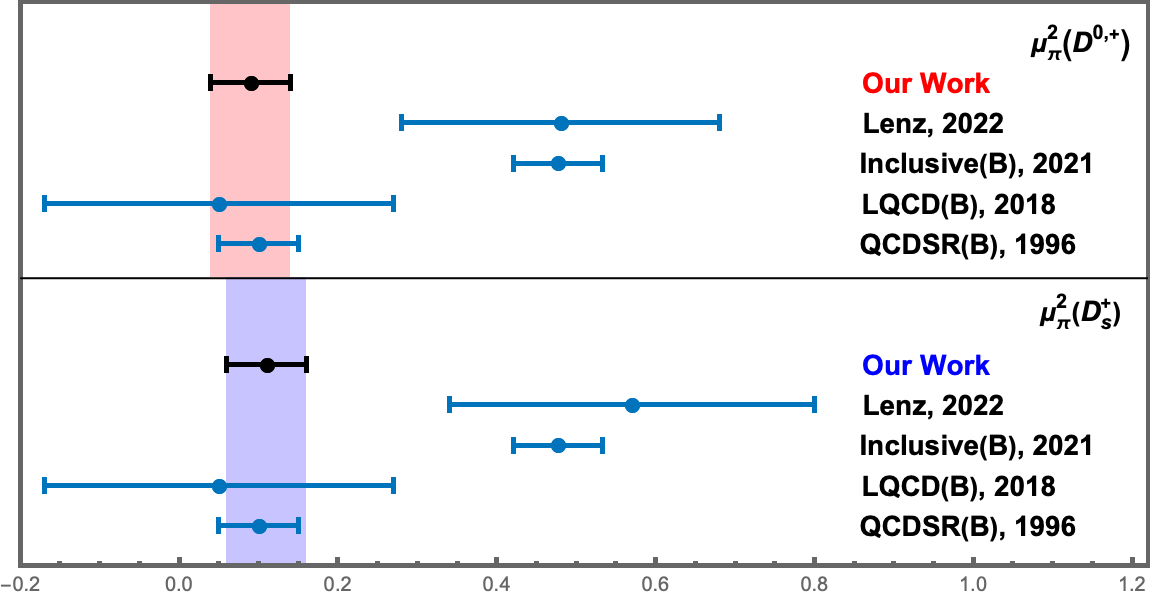
\includegraphics[width=\linewidth]{figures/mupi2.png}
          \caption{非微扰参数$\mu_{\pi}^{2}$的全局拟合估计}
          \label{fig:mupi2}
        \end{minipage}\hfill
        \begin{minipage}{0.494\textwidth}
          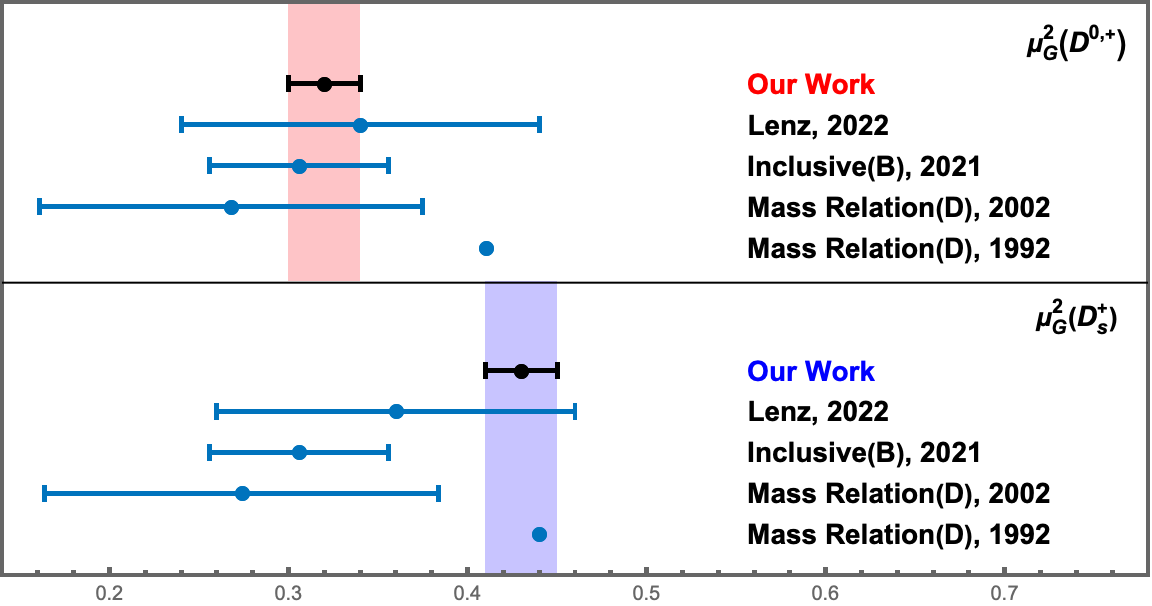
\includegraphics[width=\linewidth]{figures/mug2.png}
          \caption{非微扰参数$\mu_{G}^{2}$的全局拟合估计}
          \label{fig:mug2}
        \end{minipage}
      \end{figure}

    \subsubsection{三. 唯象学分析的结果讨论}
    上节讨论了非微扰参数的全局拟合估计并将其与底介子相关的非微扰矩阵元进行对比。本文在重夸克质量方案的讨论中里给出了1S质量方案下衰变宽度的微扰修正级数，结果表明微扰修正具有良好的收敛行为。进一步，讨论目前拟合结果下的幂次修正展开级数的收敛行为是必要的。
    
    本文将树图水平上量纲三算符对衰变宽度的贡献归一化为一，并逐项讨论各部分修正对衰变宽度的贡献，具体地，
    \begin{equation}
        \begin{aligned}
            \mrm{\Gamma_{sl}^{D^{0,+}}}&\sim 1-0.137-0.055-0.287-0.006 \cdots,\\
            \mrm{\Gamma_{sl}^{D_s^+}}&\sim 1-0.137-0.055-0.385-0.008 \cdots,\\
        \end{aligned}
        \label{eq:decaywidth_1s}
    \end{equation}
    式\eqref{eq:decaywidth_1s}中，从左至右分别是领头阶、次领头阶和次次领头阶的微扰修正和量纲五算符算符矩阵元，量纲六算符矩阵元的幂次修正贡献。无论是幂次修正还是微扰修正，使用本文关于非微扰参数的推荐值，均表现出来良好的收敛性。为了更清楚的展示，对应的贡献如图\ref{fig:D}和\ref{fig:Ds}所示。

\begin{figure}[htbp]
  \centering
  \begin{minipage}{0.5\textwidth}
    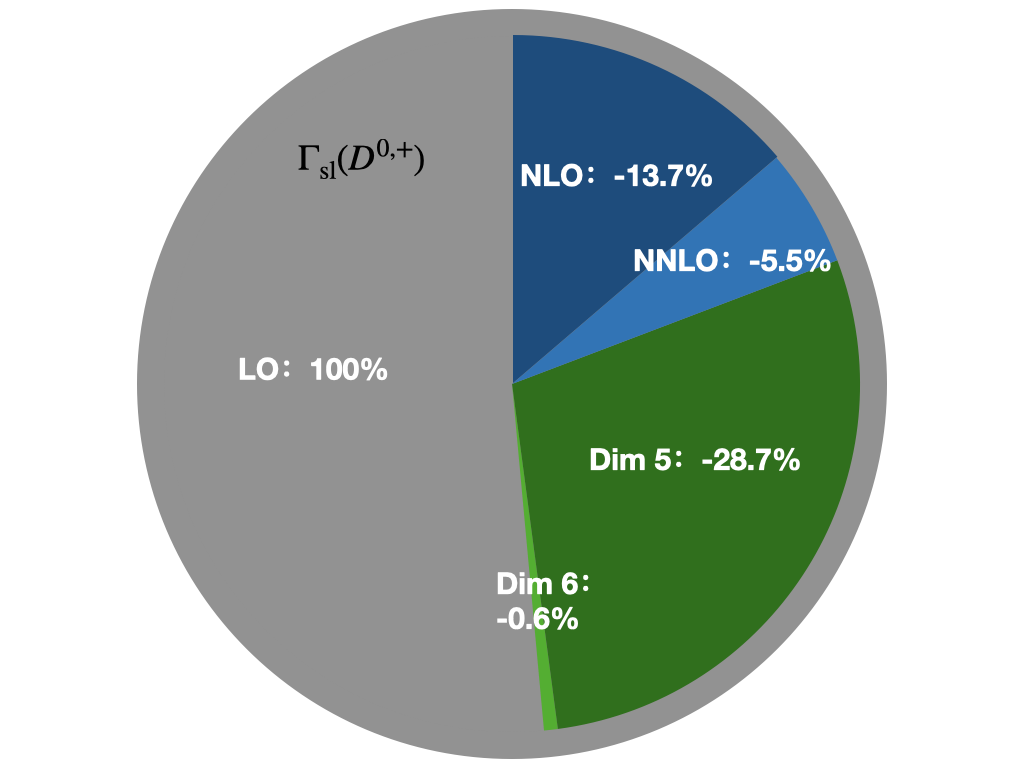
\includegraphics[width=\linewidth]{figures/D.001.png}
    \caption{$\mrm{D^{0,+}}$介子半轻单举衰宽度}
    \label{fig:D}
  \end{minipage}\hfill
  \begin{minipage}{0.5\textwidth}
    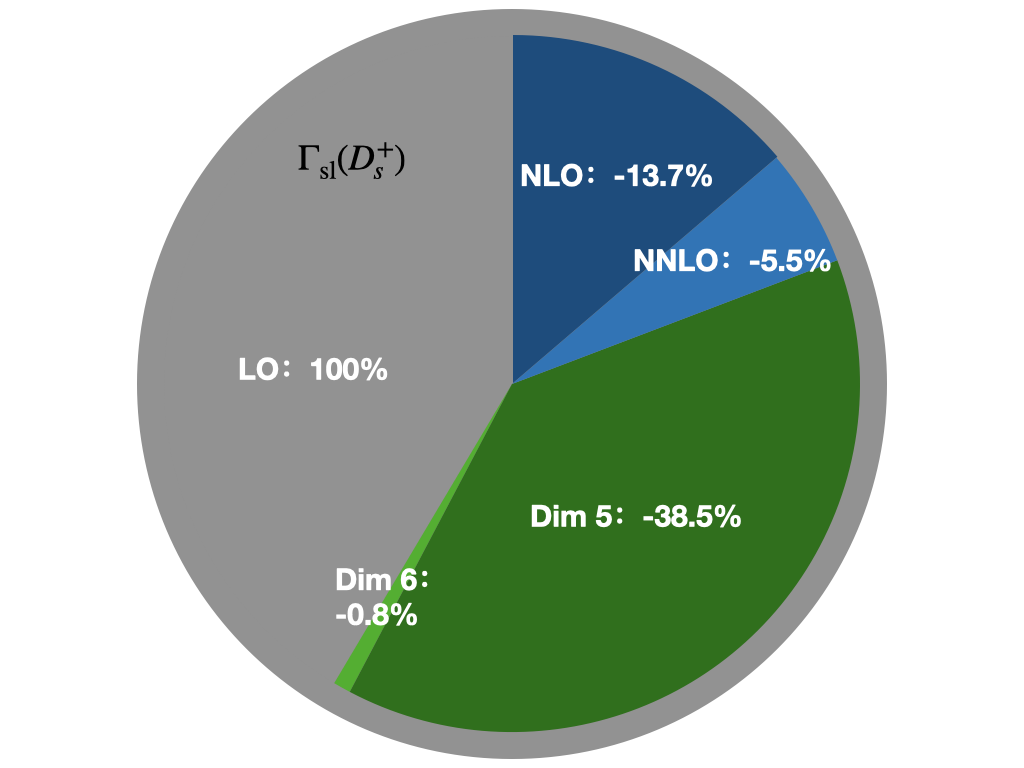
\includegraphics[width=\linewidth]{figures/Ds.001.png}
    \caption{$\mrm{D_s^+}$介子半轻单举衰宽度}
    \label{fig:Ds}
  \end{minipage}
\end{figure}


基于上述讨论，本文推荐在1S 质量方案下计算$\mrm{D}$介子衰变宽度。Alexander Lenz等人计算在$\mrm{D}$介子寿命\ct{King:2021xqp}，他们于重整化能标$\mu= 0.5\GeV$处基于动力学质量方案下给出了三种D介子的衰变宽度对重夸克有效理论中非微扰参数的具体依赖形式。

对于$\mrm{D^{0}}$介子，
\begin{equation}
    \begin{aligned}
    & \Gamma\left(\mrm{D^0}\right)= \Gamma_0[\underbrace{6.15}_{c_3^{\text {Lo }}}+\underbrace{2.95}_{\Delta c_3^{\text {NLO }}}-1.66 \frac{\mu_\pi^2(D)}{\mathrm{GeV}^2}+0.13 \frac{\mu_G^2(D)}{\mathrm{GeV}^2}+23.6 \frac{\rho_D^3(D)}{\mathrm{GeV}^3} \\
    &-1.60 \tilde{B}_1^q+1.53 \tilde{B}_2^q-21.0 \tilde{\epsilon}_1^q+19.2 \tilde{\epsilon}_2^q+\underbrace{0.00}_{\operatorname{dim}-7, \mathrm{VIA}} \\
    &\left.-10.7 \tilde{\delta}_1^{q q}+1.53 \tilde{\delta}_2^{q q}+54.6 \tilde{\delta}_3^{q q}+0.13 \tilde{\delta}_4^{q q}-29.2 \tilde{\delta}_1^{s q}+28.8 \tilde{\delta}_2^{s q}+0.56 \tilde{\delta}_3^{s q}+2.36 \tilde{\delta}_4^{s q}\right] \\
    &= 6.15 \Gamma_0\left[1+0.48-0.13 \frac{\mu_\pi^2(D)}{0.48 \mathrm{GeV}^2}+0.01 \frac{\mu_G^2(D)}{0.34 \mathrm{GeV}^2}+0.31 \frac{\rho_D^3(D)}{0.082 \mathrm{GeV}^3}\right. \\
    &-\underbrace{0.01}_{\operatorname{dim-6,\mathrm {VIA}}}-0.005 \frac{\delta \tilde{B}_1^q}{0.02}+0.005 \frac{\delta \tilde{B}_2^q}{0.02}+0.137 \frac{\tilde{\epsilon}_1^q}{-0.04}-0.125 \frac{\tilde{\epsilon}_2^q}{-0.04}+\underbrace{0.00}_{\operatorname{dim}-7, \mathrm{VIA}} \\
    &-0.0045 r_1^{q q}-0.0004 r_2^{q q}-0.0035 r_3^{q q}+0.0000 r_4^{q q} \\
    &\left.-0.0109 r_1^{s q}-0.0079 r_2^{s q}-0.0000 r_3^{s q}+0.0001 r_4^{s q}\right] .
    \end{aligned}
    \label{eq:decaywidth_D0_kinetic}
    \end{equation}
    为讨论各个部分的贡献，Lenz等人将其归一化至他们采用的中心值上。此外，他们引入$\tilde{B}_i^q = 1 + \delta \tilde{B}_i^q$以表示与真空插入近似的偏差，并且保守地将$\delta \tilde{B}_i^q$归一化为0.02。色八重算符的矩阵元素被归一化为-0.04，除此之外，还引入了比值$r_i^{q q^{\prime}} \equiv \bar{\delta}_i^{q q^{\prime}}/\langle \bar{\delta}_i^{q q^{\prime}}\rangle$表征高量纲算符的误差贡献。
    
    对于$\mrm{D^{+}}$介子，
    \begin{equation}
        \begin{aligned}
        & \Gamma\left(\mrm{D^{+}}\right)= \Gamma_0[\underbrace{6.15}_{c_3^{\mathrm{LO}}}+\underbrace{2.95}_{\Delta c_3^{\mathrm{NLO}}}-1.66 \frac{\mu_\pi^2(D)}{\mathrm{GeV}^2}+0.13 \frac{\mu_G^2(D)}{\mathrm{GeV}^2}+23.6 \frac{\rho_D^3(D)}{\mathrm{GeV}^3} \\
        &-16.9 \tilde{B}_1^q+0.56 \tilde{B}_2^q+84.0 \tilde{\epsilon}_1^q-1.34 \tilde{\epsilon}_2^q+\underbrace{6.76}_{\operatorname{dim}-7} \\
        &\left.-0.06 \tilde{\delta}_1^{q q}+0.06 \tilde{\delta}_2^{q q}-16.8 \tilde{\delta}_3^{q q}+16.9 \tilde{\delta}_4^{q q}-29.3 \tilde{\delta}_1^{s q}+28.8 \tilde{\delta}_2^{s q}+0.56 \tilde{\delta}_3^{s q}+2.36 \tilde{\delta}_4^{s q}\right] \\
        &= 6.15 \Gamma_0\left[1+0.48-0.13 \frac{\mu_\pi^2(D)}{0.48 \mathrm{GeV}^2}+0.01 \frac{\mu_G^2(D)}{0.34 \mathrm{GeV}^2}+0.31 \frac{\rho_D^3(D)}{0.082 \mathrm{GeV}^3}\right. \\
        &-\underbrace{2.66}_{text {dim-6,VIA }}-0.055 \frac{\delta \tilde{B}_1^q}{0.02}+0.002 \frac{\delta \tilde{B}_2^q}{0.02}-0.546 \frac{\tilde{\epsilon}_1^q}{-0.04}+0.009 \frac{\tilde{\epsilon}_2^q}{-0.04}+\underbrace{1.10}_{\operatorname{dim}-7, \mathrm{VIA}} \\
        &-0.0000 r_1^{q q}-0.0000 r_2^{q q}+0.0011 r_3^{q q}+0.0008 r_4^{q q} \\
        &\left.-0.0109 r_1^{s q}-0.0080 r_2^{s q}-0.0000 r_3^{s q}+0.0001 r_4^{s q}\right].
        \end{aligned}
        \label{eq:decaywidth_Dp_kinetic}
        \end{equation}
        其中，由于泡利干涉项的存在，衰变宽度中出现了巨大的负修正；，基于VIA，微扰修正与量纲六、七算符的贡献几乎相互抵消，这表明衰变宽度的展开级数对 $\mrm{\Gamma(D^{+})}$ 对高幂次算符及其QCD修正高度敏感，比如量纲五算符的QCD修正。
        \begin{equation}
            \begin{aligned}
            \Gamma\left(\mrm{D_s^{+}}\right)= & \Gamma_0[\underbrace{6.15}_{c_3^{\mathrm{LO}}}+\underbrace{2.95}_{\Delta c_3^{\mathrm{NLO}}}-1.66 \frac{\mu_\pi^2\left(D_s\right)}{\mathrm{GeV}^2}+0.13 \frac{\mu_G^2\left(D_s\right)}{\mathrm{GeV}^2}+23.6 \frac{\rho_D^3\left(D_s\right)}{\mathrm{GeV}^3} \\
            & -49.6 \tilde{B}_1^s+48.4 \tilde{B}_2^s-13.7 \tilde{\epsilon}_1^s+18.8 \tilde{\epsilon}_2^s+\underbrace{0.63}_{\operatorname{dim-7}} \\
            & \left.-15.8 \tilde{\delta}_1^{q s}+2.34 \tilde{\delta}_2^{q s}+55.4 \tilde{\delta}_3^{q s}+25.0 \tilde{\delta}_4^{q s}\right] \\
            = & 6.15 \Gamma_0\left[1+0.48-0.15 \frac{\mu_\pi^2\left(D_s\right)}{0.57 \mathrm{GeV}^2}+0.01 \frac{\mu_G^2\left(D_s\right)}{0.36 \mathrm{GeV}^2}+0.46 \frac{\rho_D^3\left(D_s\right)}{0.119 \mathrm{GeV}^3}\right. \\
            & -\underbrace{0.20}_{\text {dim-6,VIA }}-0.161 \frac{\delta \tilde{B}_1^s}{0.02}+0.157 \frac{\tilde{B}_2^s}{0.02}+0.089 \frac{\tilde{\epsilon}_1^s}{-0.04}+0.122 \frac{\tilde{\epsilon}_2^s}{0.04}+\underbrace{0.10}_{\text {dim-7,VIA }} \\
            & \left.-0.0064 r_1^{q s}-0.0007 r_2^{q s}-0.0036 r_3^{q s}+0.0012 r_4^{q s}\right]. \\
            &
            \end{aligned}
            \label{eq:decaywidth_Ds_kinetic}
            \end{equation}
        同样的，对于$\mrm{D_s^+}$介子衰变宽度也存在一组收敛性较好的微扰修正展开级数。尽管式\eqref{eq:decaywidth_D0_kinetic},式\eqref{eq:decaywidth_Dp_kinetic}和式\eqref{eq:decaywidth_Ds_kinetic}是基于动力学质量方案下给出的结果，但量纲五算符和量纲六算符的非微扰矩阵元同样起到举足轻重的作用，因此有必要将本文关于非微扰参数的抽取结果带入相关的表达式，粗略定性地展示其对寿命计算的影响。

        事实上，高量纲算符矩阵元的参数化存在模型（近似）依赖，本文将展示在重夸克有效理论求和规则（Heavy Quark Effective Theory SumRule，HQETSR）和真空插入近似两种参数化下有关D介子寿命的理论计算，
        
        Bag参数在HQETSR下的具体数值\ct{Kirk:2017juj}\ct{King:2021jsq}如表\ref{tab:bag_HQETSR}和\ref{tab:bag_HQETSR2}所示，
        \begin{table}
            \scriptsize
            \centering
        \begin{tabular}{|c||c|c|c|c|}
            \hline HQET, $\mu_0=1.5 \mathrm{GeV}$ & $\tilde{B}_1$ & $\tilde{B}_2$ & $\tilde{\epsilon}_1$ & $\tilde{\epsilon}_2$ \\
            \hline$D^{+, 0}$ & $1.0026_{-0.0106}^{+0.0198}$ & $0.9982_{-0.0066}^{+0.0052}$ & $-0.0165_{-0.0346}^{+0.0209}$ & $-0.0004_{-0.0326}^{+0.0200}$ \\
            \hline$D_s^{+}$ & $1.0022_{-0.0099}^{+0.0185}$ & $0.9983_{-0.0067}^{+0.0052}$ & $-0.0104_{-0.0330}^{+0.0202}$ & $0.0001_{-0.0324}^{+0.0199}$ \\
            \hline
            \end{tabular}
            \caption{通过HQETSR计算得到的Bag参数数值结果1}
        \label{tab:bag_HQETSR}
        \end{table}
        \begin{table}
            \scriptsize
            \centering
            \begin{tabular}{|c||c|c|c|c|}
                \hline HQET, $\mu_0=1.5 \mathrm{GeV}$ & $\tilde{\delta}_1$ & $\tilde{\delta}_2$ & $\tilde{\delta}_3$ & $\tilde{\delta}_4$ \\
                \hline$\left\langle D_q\right| \tilde{O}^q\left|D_q\right\rangle$ & $0.0026_{-0.0092}^{+0.0142}$ & $-0.0018_{-0.0072}^{+0.0047}$ & $-0.0004_{-0.0024}^{+0.0015}$ & $0.0003_{-0.0008}^{+0.0012}$ \\
                \hline$\left\langle D_s\right| \tilde{O}^q\left|D_s\right\rangle$ & $0.0025_{-0.0093}^{+0.0144}$ & $-0.0018_{-0.0072}^{+0.0047}$ & $-0.0004_{-0.0024}^{+0.0015}$ & $0.0003_{-0.0008}^{+0.0012}$ \\
                \hline$\left\langle D_q\right| \tilde{O}^s\left|D_q\right\rangle$ & $0.0023_{-0.0091}^{+0.0140}$ & $-0.0017_{-0.0070}^{+0.0046}$ & $-0.0004_{-0.0023}^{+0.0015}$ & $0.0003_{-0.0008}^{+0.0012}$ \\
                \hline
                \end{tabular}
            \caption{通过HQETSR计算得到的Bag参数数值结果2}
            \label{tab:bag_HQETSR2}
        \end{table}
        由于本文未讨论上述非微扰参数估计值之间的关联，因此这里仅讨论D介子衰变宽度理论预言的中心值。本文分析了两种情况，第一种情况对应于D介子衰变宽度的量纲五算符非微扰参数采用本文推荐值，其中非微扰参数使用Lenz等人的推荐值和HQETSR的结果；第二种情况对应于量纲五算符非微扰矩阵元以及量纲六算符的两夸克算符非微扰矩阵元采用本文推荐值，其余非微扰参数采用Lenz等人的推荐值和HQETSR的数值结果。结果如图\ref{fig:HQET}所示。
        \begin{figure}[htbp]
            \centering
            \begin{minipage}{0.5\textwidth}
              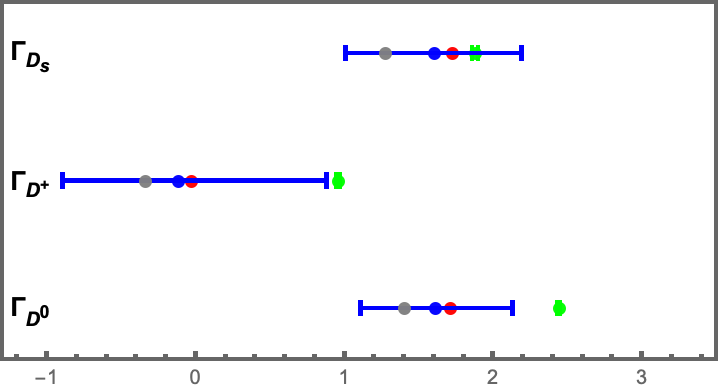
\includegraphics[width=\linewidth]{figures/HQETSR.png}
              \caption{动力学质量方案下基于HQETSR对粲介子衰变宽度的理论预言}
              \label{fig:HQET}
            \end{minipage}\hfill
            \begin{minipage}{0.5\textwidth}
              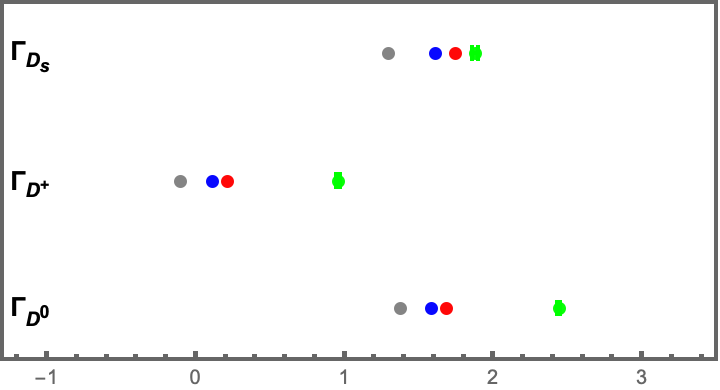
\includegraphics[width=\linewidth]{figures/VIA.png}
              \caption{动力学质量方案下基于VIA对粲介子衰变宽度的理论预言}
              \label{fig:VIA}
            \end{minipage}
          \end{figure}

        图\ref{fig:HQET}中，绿色误差棒表示BESIII合作组和CLEO合作组关于D介子的实验测量值，蓝色误差棒表示Alex Lenz等关于粲介子衰变宽度的理论计算结果，由于$\mrm{D^{+}}$介子中泡利干涉项很大的负贡献导致其理论预言的中心值小于零，且理论预言的误差远远大于实验测量值的误差且其中心值和实验观测量之间存在明显的偏离。红点对应于本文分析的第一种情况，灰点对应于本文分析的第二种情况。红点较之蓝色误差棒更靠近实验观测量值，尤其是$\mrm{D^{+}}$介子，蓝色误差棒的中心值是$-0.15/\text{ps}^{-1}$而红点将这一数值移动至$-0.03/\text{ps}^{-1}$。值得注意的是，对于本文分析的第二种情况，灰点与实验值之间存在更明显的偏离。这表明由于有限的物理可观测量导致无法实现量纲六算符夸克算符非微扰矩阵元的有效拟合估计，另一方面，体现出高幂次修正的重要性。

        此外，本文在动力学质量方案下基于VIA对粲介子寿命进行粗略定性预言，如图\ref{fig:VIA}所示。其中绿色的误差棒表示BESIII合作组和CLEO合作组关于D介子衰变宽度的测量值，蓝点表示Lenz等人基于VIA对粲介子衰变宽度的理论预言，红点对应于本文分析的第一种情况，灰点对应于我们分析的第二种情况。数据点之间的基本特征图\ref{fig:HQET}保持一致。这说明了本文实现了对量纲五算符非微扰矩阵元的有效拟合估计，且实验数据更偏向于本文关于量纲五算符非微扰参数的推荐值。

        不可否认的是，量纲六算符矩阵元的幂次修正贡献同样对粲介子衰变宽度的理论预言起到举足轻重的作用，因此未来关于高幂次算符非微扰矩阵元的QCD修正及其拟合抽取工作是必要的。
\section{本章回顾}
基于第三章关于$\mrm{D}\to X e^{+}\nu$过程的理论分析，本章从两方面介绍了D介子半轻单举衰变的唯象学分析，分别是数据抽取和唯象学分析。
\begin{itemize}
    \item [一] 数据抽取：本文从CLEO合作组$\mrm{D}\to X e^{+}\nu$的实验室系下电子能谱出发利用MC技术抽取出$\mrm{D}^0$和$\mrm{D}^+$介子的衰变宽度，电子能量一、二、三、四阶中心矩的实验观测值，$\mrm{D}_{\mrm{s}}$介子的衰变宽度，电子能量一、二、三、四阶中心矩的抽取来源于BESIII合作组的数据。此外，本文基于关联矩阵和视觉检查实现对该组观测量之间关联程度的讨论，并引入一组新观测量（衰变宽度、电子能量一阶矩与二三四阶中心矩），新观测量将与对应的物理公式一齐参与全局拟合。
    \item [二] 唯象学分析：由于物理可观测量理论公式对粲夸克质量非常敏感，因此本文基于三种质量方案实现重夸克有效理论基本参数的全局拟合抽取；对于幂次修正带来关于非微扰参数拟合估计的误差，本文在三种质量方案的基础上基于两种情形进行全局拟合估计：理论表达式截断于量纲五算符非微扰矩阵元贡献与截断于量纲六算符非微扰矩阵元贡献。对于理论输入参数误差对非微扰参数拟合估计误差的贡献，本文基于MC技术仅讨论了由于重整化能标$\mu$的跑动引起强相互作用耦合常数$\alpha_s(\mu)$的跑动对于非微扰参数拟合估计的误差贡献。
    \item [三] 结果表明：1S质量方案下精确至量纲六算符非微扰矩阵元贡献情形下的平均最小$\chi^2$最小，非微扰参数的拟合估计值没有明显的粲夸克质量方案依赖。
\end{itemize}

本文推荐1S质量方案下精确至量纲六算符非微扰矩阵元贡献情形下的非微扰参数拟合估计值作为唯象学分析的结果，此外，本文基于唯象学分析结果讨论了D介子半轻单举衰变幂次修正和微扰修正的收敛行为，发现在1S质量方案下，D介子半轻单举衰变表现出极好的收敛性。因此本文推荐在1S质量方案下对D介子寿命进行理论计算。